%!TEX root = edance.tex
%%%%%%%%%%%%%%%%
%   CHAPTER 1  %
%%%%%%%%%%%%%%%%
\chapter{Linear Time-Invariant Systems}
\label{ch:ch01_LTI}
\graphicspath{{./figs_LTI/}}
%%%%%%%%%%%%%%%%%%%%%%%%%%%%%%%%%%%%%%%%%%%%%%%%%%%%%%%%%%%%%%%%%%%%%%%%%%%%%%%%%%%%%%%%
%%%%%%%%%%%%%%%%%%%%%%%%%%%%%%%%%%%%%%%%%%%%%%%%%%%%%%%%%%%%%%%%%%%%%%%%%%%%%%%%%%%%%%%%
%                                   SECTION 1.1                                        %
%%%%%%%%%%%%%%%%%%%%%%%%%%%%%%%%%%%%%%%%%%%%%%%%%%%%%%%%%%%%%%%%%%%%%%%%%%%%%%%%%%%%%%%%
%%%%%%%%%%%%%%%%%%%%%%%%%%%%%%%%%%%%%%%%%%%%%%%%%%%%%%%%%%%%%%%%%%%%%%%%%%%%%%%%%%%%%%%%
\section{Chapter Preview}
In this chapter we will review linearity in the context of an Linear Time-Invariant (LTI) system by making analogies with discrete finite dimensional systems.  Many people have familiarity with concepts such as orthogonality and eigenfunctions from linear algebra.  It's not critical to have this background, so these references can be skipped.  Most importantly, we will show that complex exponential functions are eigenfunctions of linear systems and they span the space of solutions.  We will define the time-domain impulse response and convolution operator, and in a very natural way show the relation between the impulse response and the transfer function in the frequency domain.  This will lead us into a preview of the frequency domain representation of linear systems, which we'll pick up in the next chapter.
%%%%%%%%%%%%%%%%%%%%%%%%%%%%%%%%%%%%%%%%%%%%%%%%%%%%%%%%%%%%%%%%%%%%%%%%%%%%%%%%%%%%%%%%
%%%%%%%%%%%%%%%%%%%%%%%%%%%%%%%%%%%%%%%%%%%%%%%%%%%%%%%%%%%%%%%%%%%%%%%%%%%%%%%%%%%%%%%%
%                                   SECTION 1.2                                        %
%%%%%%%%%%%%%%%%%%%%%%%%%%%%%%%%%%%%%%%%%%%%%%%%%%%%%%%%%%%%%%%%%%%%%%%%%%%%%%%%%%%%%%%%
%%%%%%%%%%%%%%%%%%%%%%%%%%%%%%%%%%%%%%%%%%%%%%%%%%%%%%%%%%%%%%%%%%%%%%%%%%%%%%%%%%%%%%%%
\section{Example:  Analyzing an RLC Circuit}
%%%%%%%%%%%%%%%%%%%%%%%%%%%%%%%%%%%%%%%%%%%%
%             SUBSECTION 1.2.1             %
%%%%%%%%%%%%%%%%%%%%%%%%%%%%%%%%%%%%%%%%%%%%
\subsection{Example:  Low Pass Filter (LPF)}
Let's begin with an example calculation.  Suppose we have a \textbf{low pass filter}\index{Filters!Low pass} as shown in \emph{Fig.~\ref{fig:lpf}}.
%%%%%%%%%%%%%%%%%%%%%%%%%%%%%%%%%%%%%%%%%%%%
%                 FIGURE                   %
%%%%%%%%%%%%%%%%%%%%%%%%%%%%%%%%%%%%%%%%%%%%
\begin{figure}[tb]
\centering
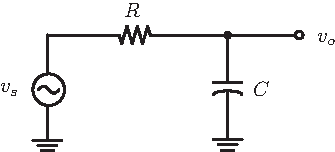
\includegraphics[scale=1]{lpf}
\caption{A simple $RC$ low-pass filter.}
\label{fig:lpf}
\end{figure}
%%%%%%%%%%%%%%%%%%%%%%%%%%%%%%%%%%%%%%%%%%%%
If we drive this system with a source $v_s$ and observe the output at $v_o$, we can write the governing equations as follows by using KVL around the loop:
    \begin{align*}
        v_o(t) &= v_s(t) - v_r(t)\\
        &= v_s(t) - i(t) R
    \end{align*}
Recall the current in a capacitor:
    \begin{equation}
        i(t) = C \frac{dv_c(t)}{dt} \label{eq:cap_curr}
    \end{equation}
Since the current is the same through the resistor and capacitor, and the voltage at the output is the same as the voltage across the capacitor, we have:
    \begin{equation*}
        v_o(t) = v_s(t) - RC \frac{dv_o(t)}{dt}
    \end{equation*}
Or, in terms of the circuit time constant $\tau = RC$:
    \begin{equation}
        v_o(t) = v_s(t) - \tau \frac{dv_o(t)}{dt} \label{eq:lpf_diff}
    \end{equation}
Let's suppose that the input signal is given by $v_s(t) = V_s \cos(\omega t)$.  We know that in steady-state  the output amplitude and phase will change: 
    \begin{equation}
        v_o(t) = \underbrace{K \cdot V_s}_{V_o} \cos(\omega t + \phi) \label{eq:kvl1}
    \end{equation}  
How do we find the change in the amplitude and phase of the signal?
%%%%%%%%%%%%%%%%%%%%%%%%%%%%%%%%%%%%%%%%%%%%
%             SUBSECTION 1.2.2             %
%%%%%%%%%%%%%%%%%%%%%%%%%%%%%%%%%%%%%%%%%%%%
\subsection{LPF the "hard way"}
The following is the wrong way to solve the problem.  It's important to review it to see how painful it can be even for a simple example.  We start by plugging the known form of the output(\emph{Eq.~\ref{eq:kvl1}}) into the LHS of the governing equation(\emph{Eq.~\ref{eq:lpf_diff}}), and verify that it satisfies the equation:
    \begin{align*}
        V_o \cos(\omega t + \phi) &= v_s(t) - \tau \frac{d}{dt}\bigg( v_o(t) \bigg)\\
        &= V_s \cos(\omega t) - \tau \frac{d}{dt}\bigg( V_o \cos(\omega t + \phi) \bigg)
            &\text{\emph{Substituting for $v_s(t)$ and $v_o(t)$}}\\
        &= V_s \cos(\omega t) + \tau \omega V_o \sin(\omega t + \phi)
    \end{align*}
Rearranging, we have:
    \begin{equation}
        V_s \cos(\omega t) = V_o \cos(\omega t + \phi) - \tau \omega V_o \sin(\omega t + \phi) \label{eq:kvl2}
    \end{equation}
Recall the following trigonometric identities:
    \begin{align*}
        \cos(x + y) &= \cos x \cos y - \sin x \sin y &\text{\emph{Sum of angles for cosine}}\\
        \sin(x + y) &= \sin x \cos y + \cos x \sin y &\text{\emph{Sum of angles for sine}}
    \end{align*}
Applying the identities to \emph{Eq.~\ref{eq:kvl2}}:
    \begin{align*}
        V_s \cos(\omega t) &= V_o \big(\cos \omega t \cos \phi - \sin \omega t \sin \phi \big)
            - \tau \omega V_o \big( \sin \omega t \cos \phi + \cos \omega t \sin \phi \big)\\
        &= V_o \cos \omega t \cos \phi - V_o \sin \omega t \sin \phi
            - V_o \tau \omega \sin \omega t \cos \phi + V_o \tau \omega \cos \omega t \sin \phi
    \end{align*}
Factoring, we have:
    \begin{equation}
        V_s \cos(\omega t) = V_o \cos(\omega t) (\cos \phi - \tau \omega \sin\phi) - V_o \sin(\omega t) (\sin\phi + \tau \omega \cos\phi)
    \end{equation}
Since sine and cosine are linearly independent\footnote{See Appendix B for a review of linear dependence/independence, and a proof for sine and cosine are LI.} functions:
    \begin{equation}
        a_1 \sin(\omega t) + a_2 \cos(\omega t) = 0
    \end{equation}
This implies that $a_1 = 0$ and $a_2 = 0$ must be zero independently.  Applying the linear independence gives us
    \begin{equation}
        -V_o \sin\phi - V_o \tau \omega \cos \phi = 0
    \end{equation}
and
    \begin{equation}
        \tan \phi = -\tau \omega
    \end{equation}
The phase response is therefore 
    \begin{equation}
        \phi = - \tan^{-1} \tau \omega
    \end{equation}
Likewise we have
    \begin{equation}
        V_o \cos\phi - V_o \tau \omega \sin\phi - V_s = 0
    \end{equation}
    \begin{equation}
        V_o (\cos \phi - \tau \omega \sin\phi) = V_s
    \end{equation}
    \begin{equation}
        V_o \cos \phi (1  - \tau \omega \tan\phi) = V_s
    \end{equation}
    \begin{equation}
        V_o \cos \phi (1  + (\tau \omega)^2 ) = V_s
    \end{equation}
    \begin{equation}
        V_o (1  + (\tau \omega)^2 )^{1/2} = V_s
    \end{equation}
 The amplitude response is therefore given by
    \begin{equation}
        \frac{V_o}{V_s} = \frac{1}{\sqrt{1 + (\tau \omega)^2}}
    \end{equation}
We can see that both the \textbf{amplitude}\index{Filters!amplitude} and \textbf{phase response}\index{Filters!phase response} are a strong function of frequency.  At very low frequencies, $\omega \approx 0$, the signal passes undisturbed.  At very high frequencies $\omega \rightarrow \infty$, the signal experiences infinite attenuation and is effectively shorted out by the capacitor.
\newpage
%%%%%%%%%%%%%%%%%%%%%%%%%%%%%%%%%%%%%%%%%%%%
%              SUB-SUBSECTION              %
%%%%%%%%%%%%%%%%%%%%%%%%%%%%%%%%%%%%%%%%%%%%
\subsubsection{LPF Magnitude and Phase Response}
%%%%%%%%%%%%%%%%%%%%%%%%%%%%%%%%%%%%%%%%%%%%
Plots of the magnitude and phase response are shown in \emph{Fig.~\ref{fig:magphase}}.  The magnitude plot shows that for signal frequencies below the cutoff frequency, $1/\tau$, the signal experiences little attenuation.  In fact, at the passband edge frequency of $1/\tau$, the magnitude is by definition lower by $1/\sqrt{2}$, which corresponds to half the power.  Likewise, the phase response is zero at low frequencies, meaning the signal is not delayed, but even at the cutoff frequency the delay is $45^\circ$, and asymptotically reaches $90^\circ$.

As is common practice in electrical engineering, we more often plot the magnitude on a log-log scale with units of dB,  as shown in \emph{Fig.~\ref{fig:magphase}}.  On the deciBel (deci = 10) scale, we take the base 10 $\log_{10}$ and multiply by $10$ to get rid of fractional parts.  The "Bel" part is in honor of the inventor of the phone,.  The dB scale allows us to expand the passband and more clearly understand the behavior of the transfer function as a function of frequency.  The multiplication by 10 is just for convenience.

But you'll notice that we often multiply log by $20$ rather than $10$ in the definition of $dB$.  Why is that?  Remember that power is proportional to voltage squared\footnote{See Appendix~\ref{sec:power_decibel} for a review of power and decibel conversions.}:
    \begin{equation}
        \mathrm{dB} = 10 \log\left( \frac{V_o}{V_s} \right)^2 = 20 \log\left( \frac{V_o}{V_s} \right)
    \end{equation}
which means that if we take the $\log$ of voltage, we can just multiply by 2 o convert it into power.
At various frequencies we have:
    \begin{equation}
        \omega = 1/\tau \rightarrow \left( \frac{V_o}{V_s} \right)_{\mathrm{dB}} = -3 \mathrm{dB}
    \end{equation}
    \begin{equation}
        \omega = 100/\tau \rightarrow \left( \frac{V_o}{V_s} \right)_{\mathrm{dB}} = -40 \mathrm{dB}
    \end{equation}
    \begin{equation}
        \omega = 1000/\tau \rightarrow \left( \frac{V_o}{V_s} \right)_{\mathrm{dB}} = -60 \mathrm{dB}
    \end{equation}
Observe that the slope of signal attenuation is 20 dB/decade in frequency beyond the passband.   Alternatively, if you double the frequency, the attenuation changes by 6 dB, or 6 dB/decade.  This is an important rule of thumb when understanding the frequency response of a system.
\newpage
%%%%%%%%%%%%%%%%%%%%%%%%%%%%%%%%%%%%%%%%%%%%
%                 FIGURE                   %
%%%%%%%%%%%%%%%%%%%%%%%%%%%%%%%%%%%%%%%%%%%%
\begin{figure}[H]
\centering
\begin{tabular}{c}
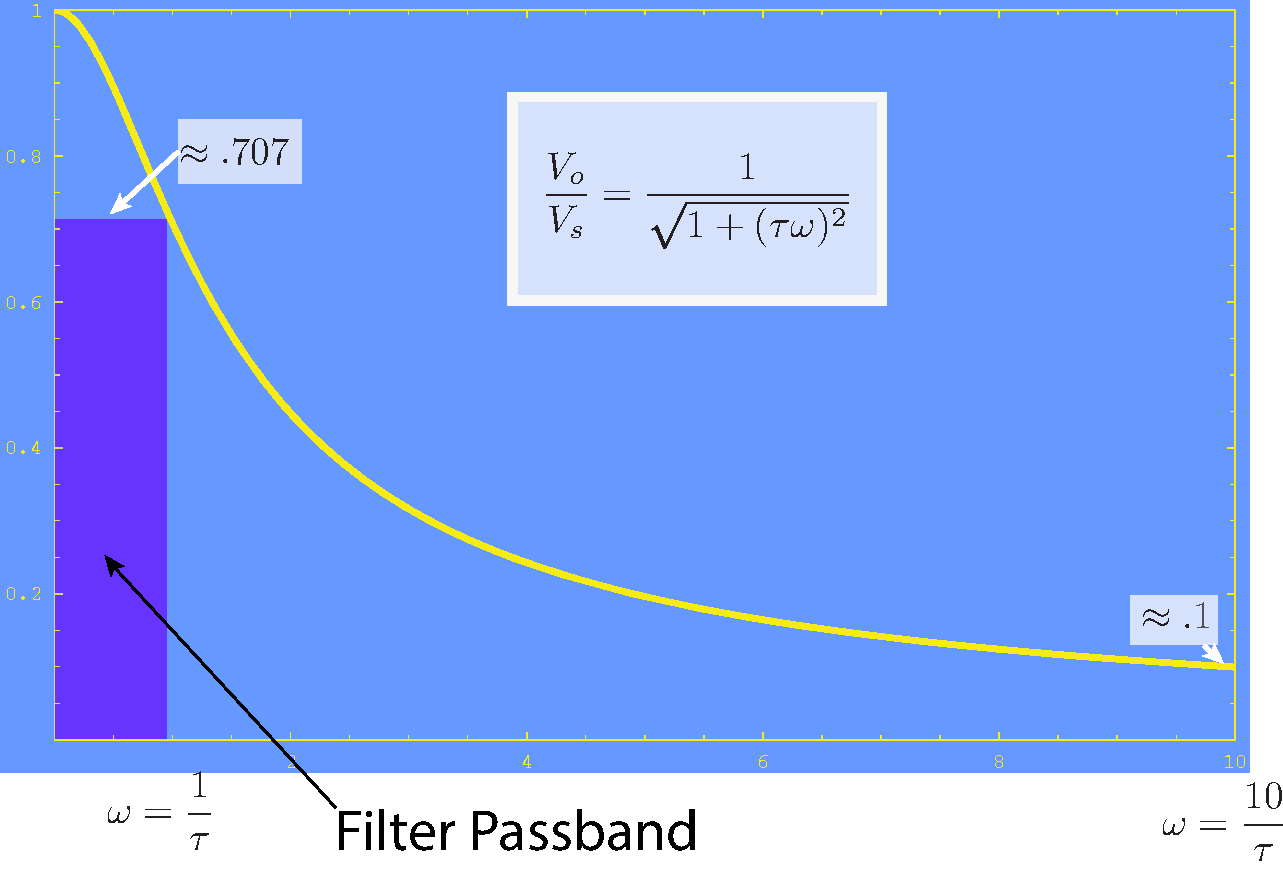
\includegraphics[width=.65\columnwidth]{mag}\\
(a)\\
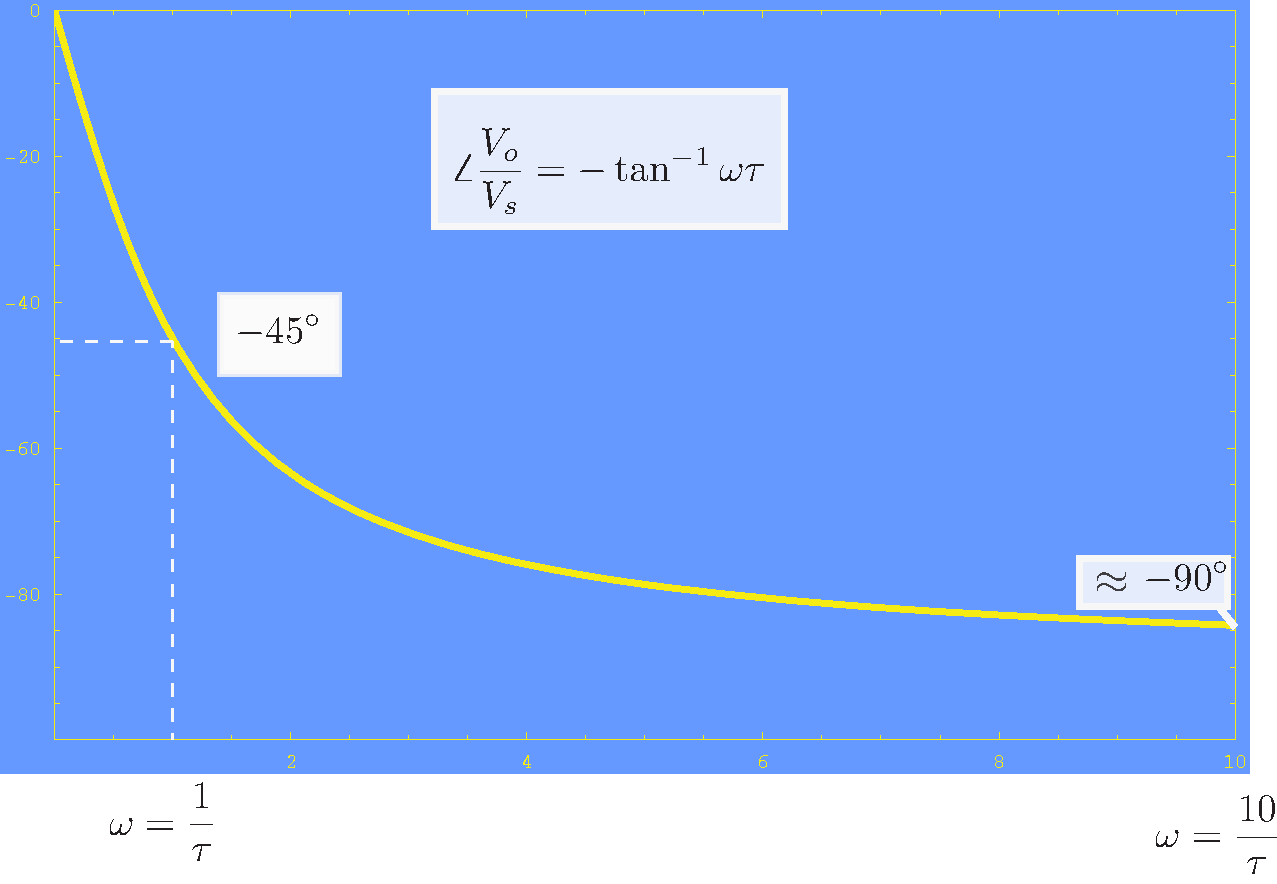
\includegraphics[width=.65\columnwidth]{phase}\\
(b)\\
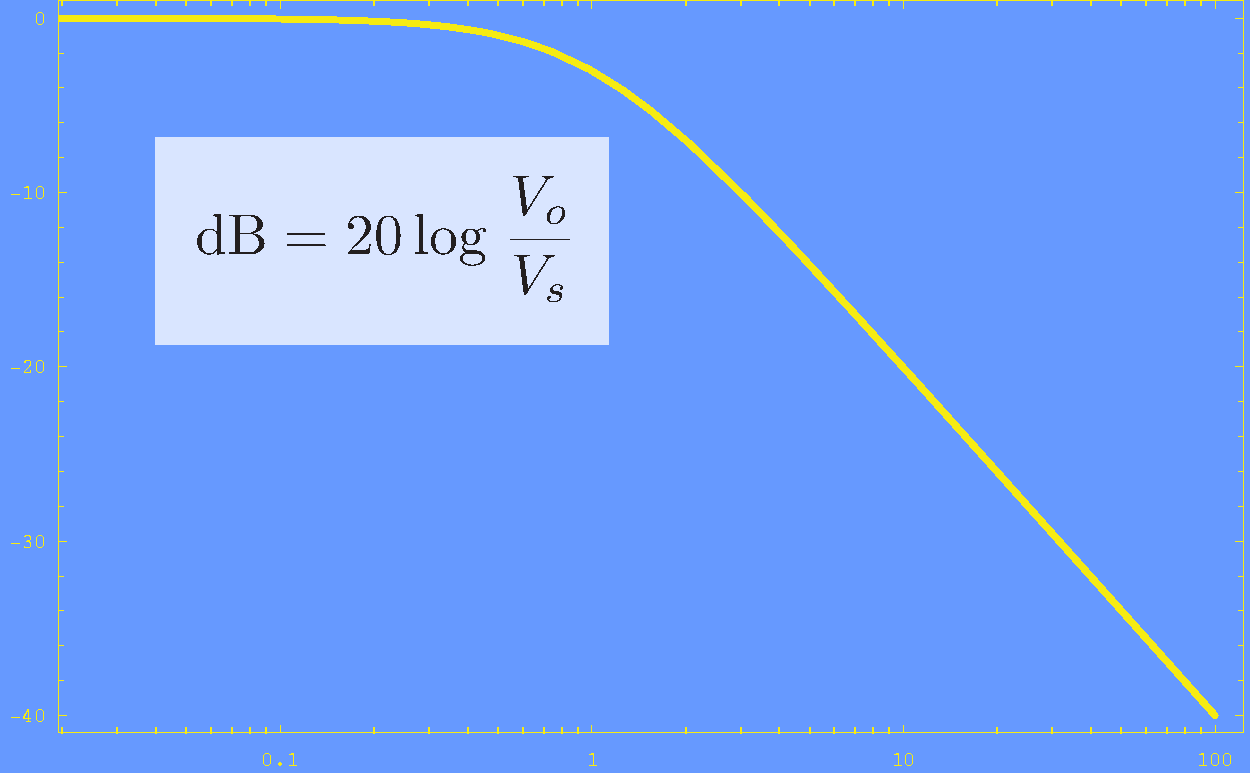
\includegraphics[width=.65\columnwidth]{dB}\\
(c)\\
\end{tabular}
\caption{The (a) magnitude and (b) phase response of the low-pass filter. The (c) log-log plot of the magnitude response of a low-pass filter (dB scale).}
\label{fig:magphase}
\end{figure}
\newpage
%%%%%%%%%%%%%%%%%%%%%%%%%%%%%%%%%%%%%%%%%%%%%%%%%%%%%%%%%%%%%%%%%%%%%%%%%%%%%%%%%%%%%%%%
%%%%%%%%%%%%%%%%%%%%%%%%%%%%%%%%%%%%%%%%%%%%%%%%%%%%%%%%%%%%%%%%%%%%%%%%%%%%%%%%%%%%%%%%
%                                   SECTION 1.3                                        %
%%%%%%%%%%%%%%%%%%%%%%%%%%%%%%%%%%%%%%%%%%%%%%%%%%%%%%%%%%%%%%%%%%%%%%%%%%%%%%%%%%%%%%%%
%%%%%%%%%%%%%%%%%%%%%%%%%%%%%%%%%%%%%%%%%%%%%%%%%%%%%%%%%%%%%%%%%%%%%%%%%%%%%%%%%%%%%%%%
\section{Linear Time-Invariant Systems}
%%%%%%%%%%%%%%%%%%%%%%%%%%%%%%%%%%%%%%%%%%%%
%             SUBSECTION 1.3.1             %
%%%%%%%%%%%%%%%%%%%%%%%%%%%%%%%%%%%%%%%%%%%%
\subsection{Linear Time-Invariant Definition}
A system $\mathbf{L}$ is linear if it satisfies the following requirement:
    \begin{equation}
        \mathbf{L} [ \alpha x(t) + \beta y(t) ] = \alpha \mathbf{L}[ x(t) ] + \beta \mathbf{L}[ y(t) ]
    \end{equation}
In this notation, $\mathbf{L}$ is an operator that corresponds to the action of the system at hand. If we input $x(t)$ an input into our system, the system outputs $y(t)$.  In a \textbf{linear system}\index{Linear systems}, if we scale the input, we also scale the output by the same amount. Also, if we take a superposition of inputs, the output is the same superposition of the inputs.

Now, a system is \textbf{time invariant}\index{Linear systems!Time invariant} if its response is not a function of time. In other words, the system does not "age" and it does not care when you apply the input.  If you apply an input today and observe the output, and come back tomorrow and put in the same input, the output should look the same.  Mathematically, we can summarize this behavior with the following equations:
    \begin{equation}
        y(t) = \mathbf{L} [x(t)]
    \end{equation}
    \begin{equation}
        \mathbf{L} [x(t-\tau)] = y(t-\tau)
    \end{equation}
Notice that \textbf{time shifting}\index{Linear systems!Time shifting} the input just corresponds to applying the same time shift to the output.  Another way to think of time-invariance is to say that the system has no  "clock" or time reference, or that the transfer function is not a function of time.  It does not matter when you apply the input.  The transfer function is going to be the same. 

 If you are familiar with discrete linear system, you know that linearity and superposition are fundamental properties. 
%%%%%%%%%%%%%%%%%%%%%%%%%%%%%%%%%%%%%%%%%%%%
%              SUB-SUBSECTION              %
%%%%%%%%%%%%%%%%%%%%%%%%%%%%%%%%%%%%%%%%%%%%
\subsubsection{Vectors and Matrices Become Functions and Integrals}
 In finite dimensional discrete linear systems, inputs and outputs are defined in terms of input and output vectors.  For LTI systems, we can think of the inputs and outputs as infinite dimensional vectors, but instead of a countably infinite set of elements we have a uncountably large number of time instants that define the input and output.  In other words, we represent the input and output as continuous functions of time.   We will see that in LTI systems, we can also represent linear systems by basis functions:
    \begin{equation}
        \phi_1(t), \phi_2(t), \cdots
    \end{equation}
and instead of a matrix representation (summation) we will have an integral representation called the \textbf{Convolution Integral}\index{Convolutions!integral}.  Eigenvectors have the direct analog of Eigenfunctions:
    \begin{equation}
        \mathbf{L} [  \phi_n(t)  ] = \lambda_n  \phi_n(t)
    \end{equation}
And the concept of an \textbf{Orthonormal Basis}\index{Orthonormal basis} maps directly into LTI systems:
    \begin{equation}
        x(t) = \sum_n \phi_n(t) x_n
    \end{equation}
    \begin{equation}
        x(t) = \int \phi(s t) x(t) dt
    \end{equation}
We can therefore perform \textbf{Eigenfunction}\index{Eigenfunction} expansion of an arbitrary input and study the response of a linear system to an arbitrary input by using our knowledge of how the system responds to the eigenfunctions.  In other words, the eigenvalues of the system, or the spectral expansion, will be the most important aspect of a linear system.

If this doesn't make any sense, don't worry.  We'll cover all of this in a step-by-step fashion. This is only meant as a teaser for people who have seen linear system theory previously. 
%%%%%%%%%%%%%%%%%%%%%%%%%%%%%%%%%%%%%%%%%%%%%%%%%%%%%%%%%%%%%%%%%%%%%%%%%%%%%%%%%%%%%%%%
%%%%%%%%%%%%%%%%%%%%%%%%%%%%%%%%%%%%%%%%%%%%%%%%%%%%%%%%%%%%%%%%%%%%%%%%%%%%%%%%%%%%%%%%
%                                   SECTION 1.4                                        %
%%%%%%%%%%%%%%%%%%%%%%%%%%%%%%%%%%%%%%%%%%%%%%%%%%%%%%%%%%%%%%%%%%%%%%%%%%%%%%%%%%%%%%%%
%%%%%%%%%%%%%%%%%%%%%%%%%%%%%%%%%%%%%%%%%%%%%%%%%%%%%%%%%%%%%%%%%%%%%%%%%%%%%%%%%%%%%%%%
\section{The Complex Exponential Technique}
We begin by introducing the complex exponential, and we will show that complex exponentials are eigenfunctions of linear systems.  This means that they play an immensely central role in linear system analysis.
%%%%%%%%%%%%%%%%%%%%%%%%%%%%%%%%%%%%%%%%%%%%
%             SUBSECTION 1.4.1             %
%%%%%%%%%%%%%%%%%%%%%%%%%%%%%%%%%%%%%%%%%%%%
\subsection{Why introduce complex numbers?}
Complex exponentials actually make things less complex.  To see this, first note that integration and differentiation are trivial with complex exponentials:
    \begin{equation}
        \frac{d}{dt} e^{j\omega t} = j \omega e^{j\omega t}
    \end{equation}
    \begin{equation}
        \int e^{j\omega x} dx = \frac{1}{j \omega} e^{j\omega t}
    \end{equation}
So now any ordinary \textbf{differential equation}\index{Differential equations!ordinary} (ODE), a sum of differentiation operators, is reduced now to trivial algebraic manipulations.  In fact, we'll show that you don't even need to directly derive the ODE by using \textbf{phasors}\index{Phasors} (a phasor is essentially a shorthand notation for a complex number).   The key is to observe that the current/voltage relation for any element can be derived for \textbf{complex exponential}\index{Complex exponential} excitation.
%%%%%%%%%%%%%%%%%%%%%%%%%%%%%%%%%%%%%%%%%%%%
%             SUBSECTION 1.4.2             %
%%%%%%%%%%%%%%%%%%%%%%%%%%%%%%%%%%%%%%%%%%%%
\subsection{Complex Exponential}
From Euler's we have an important relationship between complex exponentials and ordinary $\sin$ and $\cos$ functions:
    \begin{equation}
        e^{j x} = \cos x + j \sin x
    \end{equation}
If take the magnitude of this quantity, it's unity
    \begin{equation}
        | e^{j x} | = \sqrt{\cos^2 x +  \sin^2 x}  = 1
    \end{equation}
This means that for any value of $x$, the magnitude of a complex exponential is 1.  Thus,  $e^{j\phi}$ is a point on the unit circle at an angle of $\phi$ from the $x$-axis. 

Any complex number $z$ (\emph{Fig.~\ref{fig:complex}}), expressed as having a real and imaginary part $ z = x + j y$, can also be interpreted as having a magnitude and a phase.  The magnitude  $|z| = \sqrt{x^2 + y^2}$ and the phase $\phi = \angle z = \tan^{-1} y/x$ can be combined using the complex exponential
    \begin{equation}
        x + j y = |z| e^{j\phi}
    \end{equation}
%%%%%%%%%%%%%%%%%%%%%%%%%%%%%%%%%%%%%%%%%%%%
%                 FIGURE                   %
%%%%%%%%%%%%%%%%%%%%%%%%%%%%%%%%%%%%%%%%%%%%
\begin{figure}[H]
\centering
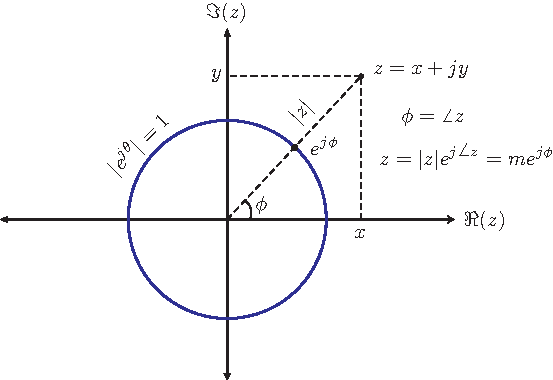
\includegraphics[width=.55\columnwidth]{complex}
\caption{A general complex number $z$ can be represented by its real and imaginary components, or its magnitude and phase.}
\label{fig:complex}
\end{figure}
%%%%%%%%%%%%%%%%%%%%%%%%%%%%%%%%%%%%%%%%%%%%
%%%%%%%%%%%%%%%%%%%%%%%%%%%%%%%%%%%%%%%%%%%%
%             SUBSECTION 1.4.3             %
%%%%%%%%%%%%%%%%%%%%%%%%%%%%%%%%%%%%%%%%%%%%
\subsection{Euler's Relations and The Circle}
The argument to $e^{j \omega t}$ is just linearly increasing with a slope of $\omega$, and completes $2\pi$ radian every $\frac{2\pi}{\omega}$ seconds.  This implies that $e^{j \omega t}$ is nothing but a point rotating on a circle on the complex plane.  The real part and imaginary parts are just projections of the circle, which by trigonometry we know equal the cosine and sine functions.

 We can also express $\cos$ and $\sin$ in terms of $e$ as follows
    \begin{equation}
        \cos x = \frac{e^{jx} + e^{-jx}}{2}
    \end{equation}
    \begin{equation}
        \sin x = \frac{e^{jx} - e^{-jx}}{2j}
    \end{equation}
which shows that two counter rotating complex exponentials sum to $\sin$ and $\cos$.  We can visualize these relations as shown in \emph{Fig.~\ref{fig:complexexp}}.  Be sure to click the links to see an animation, especially for the sum of two counter rotating complex exponentials in \emph{Fig.~\ref{fig:cos}}.
%%%%%%%%%%%%%%%%%%%%%%%%%%%%%%%%%%%%%%%%%%%%
%                 FIGURE                   %
%%%%%%%%%%%%%%%%%%%%%%%%%%%%%%%%%%%%%%%%%%%%
\begin{figure}[tb]
\centering
\begin{tabular}{cc}
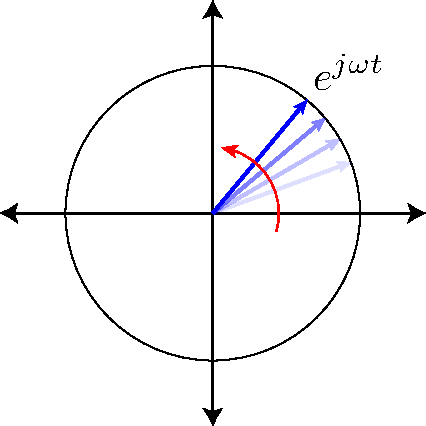
\includegraphics[width=.4\columnwidth]{exp1.pdf}  &
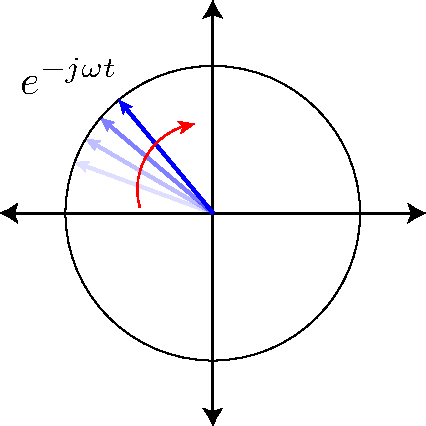
\includegraphics[width=.4\columnwidth]{exp2.pdf} \\
(a) & (b) \\
\end{tabular}
\caption{  (a) The complex exponential $e^{j\omega t}$ rotates around the unit circle counter-clockwise at a rate of $\omega$, or once every $2\pi/\omega$ seconds.  Likewise (b) $e^{-j\omega t}$ rotates around the unit circle clockwise.  Click \href{http://rfic.eecs.berkeley.edu/~niknejad/photos/ee105/exp1.mov}{$e^{j\omega t}$ \emph{here}} and \href{http://rfic.eecs.berkeley.edu/~niknejad/photos/ee105/exp2.mov}{$e^{-j\omega t}$ \emph{here}} to see the animations.}
\label{fig:complexexp}
\end{figure}
%%%%%%%%%%%%%%%%%%%%%%%%%%%%%%%%%%%%%%%%%%%%
%                 FIGURE                   %
%%%%%%%%%%%%%%%%%%%%%%%%%%%%%%%%%%%%%%%%%%%%
\begin{figure}[tb]
\centering
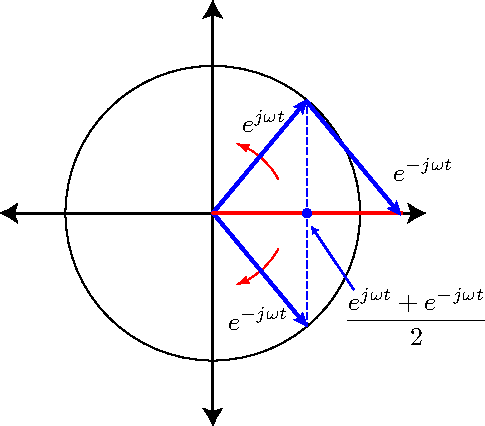
\includegraphics[width=.45\columnwidth]{exp3.pdf}
\caption{We visualize the function $\cos$ by building it through vectorwise addition of $e^{j\omega t}$ and $e^{-j\omega t}$.  Click \href{http://rfic.eecs.berkeley.edu/~niknejad/photos/ee105/exp3.mov}{\emph{here}} to see the animation.}
\label{fig:cos}
\end{figure}
%%%%%%%%%%%%%%%%%%%%%%%%%%%%%%%%%%%%%%%%%%%%
%             SUBSECTION 1.4.4             %
%%%%%%%%%%%%%%%%%%%%%%%%%%%%%%%%%%%%%%%%%%%%
\subsection{The Magic of Sinusoids}
%%%%%%%%%%%%%%%%%%%%%%%%%%%%%%%%%%%%%%%%%%%%
%                 FIGURE                   %
%%%%%%%%%%%%%%%%%%%%%%%%%%%%%%%%%%%%%%%%%%%%
\begin{figure}[tb]
\centering
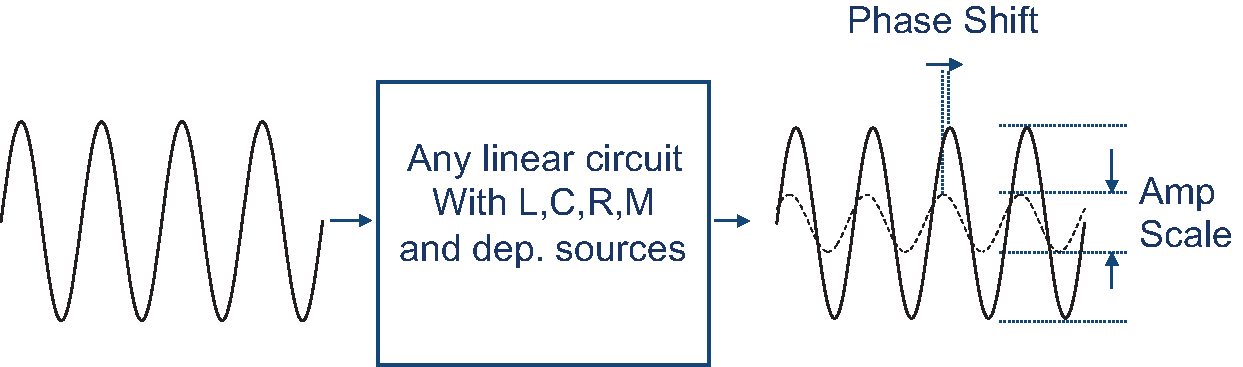
\includegraphics[width=.65\columnwidth]{lti_sine}
\caption{In an LTI system, if we drive it with a sinusoid, the output is a sinusoid at the same frequency, with a new amplitude and phase.}
\label{fig:lti_sine}
\end{figure}
%%%%%%%%%%%%%%%%%%%%%%%%%%%%%%%%%%%%%%%%%%%%
What were going to show is that when a linear, time invariant (LTI) circuit is excited by a sinusoid (see \emph{Fig.~\ref{fig:lti_sine}}), it's output is a sinusoid at the same frequency.  Only the magnitude and phase of the output differ from the input.  Sinusoids are very special functions for LTI systems, in other words they are eigenfunctions.  The \textbf{"Frequency Response''}\index{Linear systems!frequency response} is a characterization of the input-output response for sinusoidal inputs at all frequencies.

Since most periodic (non-periodic) signals can be decomposed into a summation (integration) of sinusoids via Fourier Series (Transform), the response of a LTI system to virtually any input is characterized by the frequency response of the system.  We'll return to this point later.
%%%%%%%%%%%%%%%%%%%%%%%%%%%%%%%%%%%%%%%%%%%%
%              SUB-SUBSECTION              %
%%%%%%%%%%%%%%%%%%%%%%%%%%%%%%%%%%%%%%%%%%%%
\subsubsection{Complex Exponential is Powerful}
To find steady state response we can excite the system with a complex exponential.   Here our system is any general LTI system. In terms of circuits, it is any linear circuit consisting of resistors, capacitors, inductors, mutual inductors, transformers, and linear dependent sources.  At any frequency, the system response is characterized by a single complex number $H$, as shown in \emph{Fig.~\ref{fig:lti_resp}}.   The magnitude response is given by $|H(\omega)|$ and
the phase response is given by $\angle H$.   We see that the complex exponential is an "eigenfunction" of the system.  It is used to probe the system.  If we characterize the response to all eigenfunctions, we can completely characterize the system.   Because a sinusoid is a sum of complex exponentials (and because of linearity!), we can also probe a system by applying a real sinusoidal input.  This is what we do in the lab.
%%%%%%%%%%%%%%%%%%%%%%%%%%%%%%%%%%%%%%%%%%%%
%                 FIGURE                   %
%%%%%%%%%%%%%%%%%%%%%%%%%%%%%%%%%%%%%%%%%%%%
\begin{figure}[tb]
\centering
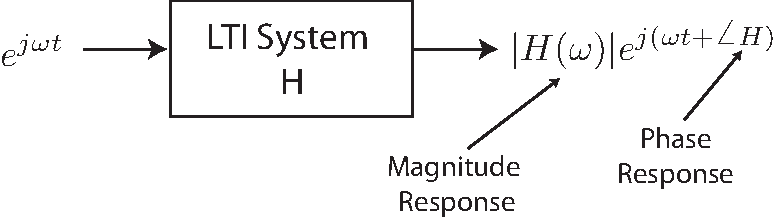
\includegraphics[width=.65\columnwidth]{lti_resp}
\caption{The complex exponential response of a linear system is another complex exponential, with an additional magnitude and phase factor. }
\label{fig:lti_resp}
\end{figure}
%%%%%%%%%%%%%%%%%%%%%%%%%%%%%%%%%%%%%%%%%%%%
%              SUB-SUBSECTION              %
%%%%%%%%%%%%%%%%%%%%%%%%%%%%%%%%%%%%%%%%%%%%
\subsubsection{$H$ is the Transfer Function}
In summary, $e^{j\omega}$ is an eigenfunction for any linear system (circuit), and $H(\omega)$ is the eigenvalue of the system.  There's a continuous spectrum of eigenvalues $H(\omega)$.   The linear system is completely characterized by the spectrum of eigenvalues, or in the frequency domain by the \textbf{transfer function}\index{Transfer function} $H(\omega)$.  We also often write $H(\omega)$ in the following form (explained shortly):
    \begin{equation}
        H(j\omega)
    \end{equation}
%%%%%%%%%%%%%%%%%%%%%%%%%%%%%%%%%%%%%%%%%%%%%%%%%%%%%%%%%%%%%%%%%%%%%%%%%%%%%%%%%%%%%%%%
%%%%%%%%%%%%%%%%%%%%%%%%%%%%%%%%%%%%%%%%%%%%%%%%%%%%%%%%%%%%%%%%%%%%%%%%%%%%%%%%%%%%%%%%
%                                   SECTION 1.5                                        %
%%%%%%%%%%%%%%%%%%%%%%%%%%%%%%%%%%%%%%%%%%%%%%%%%%%%%%%%%%%%%%%%%%%%%%%%%%%%%%%%%%%%%%%%
%%%%%%%%%%%%%%%%%%%%%%%%%%%%%%%%%%%%%%%%%%%%%%%%%%%%%%%%%%%%%%%%%%%%%%%%%%%%%%%%%%%%%%%%
\section{The Low Pass Filter Again}
%%%%%%%%%%%%%%%%%%%%%%%%%%%%%%%%%%%%%%%%%%%%
%             SUBSECTION 1.5.1             %
%%%%%%%%%%%%%%%%%%%%%%%%%%%%%%%%%%%%%%%%%%%%
\subsection{LPF Example:  The "soft way''}
Remember that earlier we tried to analyze the low-pass filter using sinusoids.  Now let's excite the system with a complex exponential.  Recall that the sinusoidal response is related to the exponential response so we can always recover the sinusoidal response from the complex exponential\index{Complex exponential} response
    \begin{equation}
        v_s(t) = v_o(t) + \tau \frac{dv_o}{dt}
    \end{equation}
Derivatives are simply products with $j\omega$
    \begin{equation}
        v_s(t) = V_s e^{j\omega t}
    \end{equation}
Grouping terms
    \begin{equation}
        v_o(t) = |V_o| e^{j (\omega t + \phi)} = V_o e^{j\omega t}
    \end{equation}
Now substitute into the original equation
    \begin{equation}
        V_s e^{j \omega t} = V_o e^{j \omega t}  + \tau \cdot j\omega \cdot V_o e^{j \omega t}
    \end{equation}
and divide out the non-zero common factors ($|e^{j\omega t} | = 1$)
    \begin{equation}
        V_s = V_o ( 1 + j \omega \cdot \tau)
    \end{equation}
So with a few lines of algebra, we have the transfer function:
    \begin{equation}
        \frac{V_o}{V_s} = \frac{1}{1 + j\omega \cdot \tau}
    \end{equation}
The system is characterized by the complex function
    \begin{equation}
        H(\omega) = \frac{V_o}{V_s} = \frac{1}{1 + j\omega \cdot \tau}
    \end{equation}
The magnitude and phase response match our previous calculation:
    \begin{equation}
        | H(\omega) | = \left|\frac{V_o}{V_s}\right| = \frac{1}{\sqrt{1 + (\omega \tau)^2}}
    \end{equation}
    \begin{equation}
        \angle H(\omega) = - \tan^{-1} \omega \tau
    \end{equation}
Clearly, using the complex exponential is much faster and easier than the earlier approach where we used sinusoids directly and the final answer is the same.  It's not obvious why the transfer function for a complex exponential matches the one for the sinusoidal excitation.  Let's explore this further.
%%%%%%%%%%%%%%%%%%%%%%%%%%%%%%%%%%%%%%%%%%%%
%              SUB-SUBSECTION              %
%%%%%%%%%%%%%%%%%%%%%%%%%%%%%%%%%%%%%%%%%%%%
\subsubsection{Why did it work?}
If we push the complex exponential through the system and take the real part of the output, then why is that the same as the "real'' sinusoidal response?  One argument to explain why the complex exponential works in place of a sinusoid is to observe that sine and cosine are simply imaginary and real parts of the complex exponential.  So any signal (current or voltage) can be written in the following equivalent forms
    \begin{equation}
        s(t) = S_o \cos(\omega t + \phi) = S_o \Re[e^{j(\omega t + \phi)}]
    \end{equation}
For example, if we excite our system with an input $z(t)$ that is complex, producing an output $y_z(t)$, and if we take the real or imaginary part of the signals, we have
    \begin{equation}
        y_z(t) = \mathbf{L}(z(t))
    \end{equation}
Now take the real part of both sides and use the fact that the order of the operator $\Re$ and our system $\mathbf{L}$ can be interchanged:
    \begin{equation}
        \Re[y_z(t)] = \Re[\mathbf{L}(z(t))]  = \mathbf{L} (\Re[z(t)])
    \end{equation}
If this argument does not convince you, there's a slightly more complicated way to show this must be true.
%%%%%%%%%%%%%%%%%%%%%%%%%%%%%%%%%%%%%%%%%%%%
%                 FIGURE                   %
%%%%%%%%%%%%%%%%%%%%%%%%%%%%%%%%%%%%%%%%%%%%
\begin{figure}[tb]
\centering
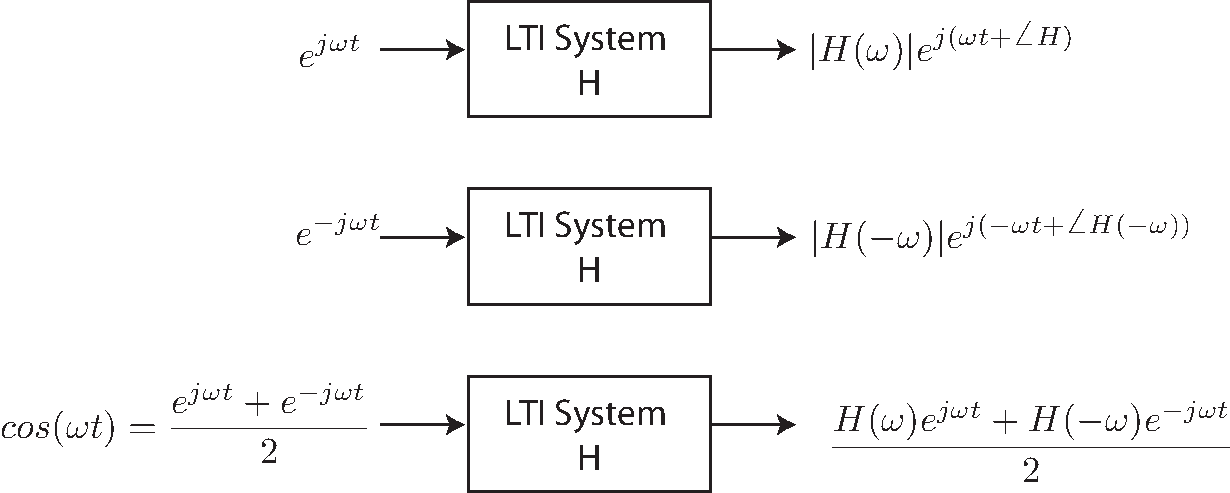
\includegraphics[width=.75\columnwidth]{lti_cosine}
\caption{Sinusoidal response of an LTI system by superposition. }
\label{fig:lti_cosine}
\end{figure}
%%%%%%%%%%%%%%%%%%%%%%%%%%%%%%%%%%%%%%%%%%%%
%              SUB-SUBSECTION              %
%%%%%%%%%%%%%%%%%%%%%%%%%%%%%%%%%%%%%%%%%%%%
\subsubsection{And yet another perspective}
As shown in \emph{Fig.~\ref{fig:lti_cosine}}, another way to see this is to observe that the system is linear so that we can push through two inputs separately and sum the outputs:
    \begin{equation}
        y = \mathbf{L}(s_1(t) + s_2(t)) = \mathbf{L}(s_1(t)) + \mathbf{L}(s_2(t))
    \end{equation}
Similarly, to find the response to a sinusoid, we can find the response to $e^{j\omega t}$ and $e^{-j\omega t}$, and sum the results.  For a linear system represented by real circuit elements, if  the input is real function of time, the output must also be a real function:
    \begin{equation}
        y(t) = \frac{H(\omega) e^{j\omega t} + H(-\omega) e^{-j\omega t} }{2}
    \end{equation}
The only way for two complex numbers to sum to a real number is if they are complex conjugates.  That means the second term is the conjugate of the first, which implies that
    \begin{equation}
        |H(-\omega)| = |H(\omega)|
    \end{equation}
Or in other words, the magnitude response is an even function of frequency.  Likewise, we have
    \begin{equation}
        \angle H(-\omega) = -\angle H(\omega) = - \phi
    \end{equation}
Or the phase function has to be an odd function of frequency.  Therefore the output is given by
    \begin{equation}
        y(t) = \frac{|H(\omega)|}{2} \left( e^{j(\omega t + \phi)} + e^{-j(\omega t + \phi)} \right)
    \end{equation}
or more simply
    \begin{equation}
        |H(\omega)| \cos(\omega t + \phi)
    \end{equation}
%%%%%%%%%%%%%%%%%%%%%%%%%%%%%%%%%%%%%%%%%%%%%%%%%%%%%%%%%%%%%%%%%%%%%%%%%%%%%%%%%%%%%%%%
%%%%%%%%%%%%%%%%%%%%%%%%%%%%%%%%%%%%%%%%%%%%%%%%%%%%%%%%%%%%%%%%%%%%%%%%%%%%%%%%%%%%%%%%
%                                   SECTION 1.6                                        %
%%%%%%%%%%%%%%%%%%%%%%%%%%%%%%%%%%%%%%%%%%%%%%%%%%%%%%%%%%%%%%%%%%%%%%%%%%%%%%%%%%%%%%%%
%%%%%%%%%%%%%%%%%%%%%%%%%%%%%%%%%%%%%%%%%%%%%%%%%%%%%%%%%%%%%%%%%%%%%%%%%%%%%%%%%%%%%%%%
\section{Generalization to any Linear Circuit}
%%%%%%%%%%%%%%%%%%%%%%%%%%%%%%%%%%%%%%%%%%%%
%             SUBSECTION 1.6.1             %
%%%%%%%%%%%%%%%%%%%%%%%%%%%%%%%%%%%%%%%%%%%%
\subsection{"Proof'' for Linear Systems}
For an arbitrary linear circuit, in other words a black box containing an arbitrary number of inductors, capacitors, resistors, mutual inductors, or linear dependent sources, we can  decompose the system into linear sub-operators, like multiplication by constants, time derivatives, or integrals:
    \begin{equation}
        y = \mathbf{L}(x) = a x + b_1 \frac{d}{dt} x + b_2\frac{d^2}{dt^2} x + \cdots + c_1 \int x + c_2 \iint x + \cdots
    \end{equation}
For a complex exponential input this simplifies to:
    \begin{equation}
        y  = \mathbf{L}(e^{j\omega t}) = a e^{j\omega t} + b_1 \frac{d}{dt} e^{j\omega t} + b_2\frac{d^2}{dt^2} e^{j\omega t} + \cdots + c_1 \int e^{j\omega t} + c_2 \iint e^{j\omega t} + \cdots
    \end{equation}
    \begin{equation}
        y  = a e^{j\omega t} + b_1 j\omega e^{j\omega t} + b_2 ( j\omega)^2 e^{j\omega t} + \cdots + c_1 \frac{e^{j\omega t}}{ j\omega} + c_2 \frac{e^{j\omega t}}{ (j\omega)^2} + \cdots
    \end{equation}
Note that every term is of the form $e^{j\omega t}$ times a constant, which when grouped together gives
    \begin{equation}
        y =  e^{j\omega t} \underbrace{\left(a  + b_1 j\omega  + b_2 ( j\omega)^2 + \cdots + c_1 \frac{1}{ j\omega} + c_2 \frac{1}{ (j\omega)^2}  + \cdots \right)}_{H}
    \end{equation}
We've grouped together all the terms multiplying $e^{j\omega t}$ and note that at a given frequency, they sum to a complex number $H$.    The amplitude of the output is the magnitude of the complex number $H$ and the phase of the output is the phase of the complex number $H$.
    \begin{equation}
        y =  e^{j\omega t} \underbrace{\left(a  + b_1 j\omega + b_2 ( j\omega)^2 + \cdots + \frac{1}{ j\omega} + \frac{1}{ (j\omega)^2}  + \cdots \right)}_{H}
    \end{equation}
Written more compactly, we have
    \begin{equation}
        y = e^{j\omega t} |H(\omega)| e^{j\angle H(\omega)}
    \end{equation}
or equivalently
    \begin{equation}
        \Re[ y ] =  |H(\omega)| \cos ( \omega t + \angle H(\omega))
    \end{equation}
%%%%%%%%%%%%%%%%%%%%%%%%%%%%%%%%%%%%%%%%%%%%
%             SUBSECTION 1.6.2             %
%%%%%%%%%%%%%%%%%%%%%%%%%%%%%%%%%%%%%%%%%%%%
\subsection{General Complex Exponential}
Looking back at our derivation, it's clear that a complex exponential is also an eigenfunction of our system, and the periodic complex exponential is just a special case.  We can make the same argument for a general input of the form $e^{st}$:
    \begin{equation}
        y = \mathbf{L}(x) = a x + b_1 \frac{d}{dt} x + b_2\frac{d^2}{dt^2} x + \cdots + c_1 \int x + c_2 \iint x + \cdots
    \end{equation}
    \begin{equation}
        y =  e^{s t} \underbrace{\left(a + b_1 s  + b_2 s^2  + \cdots + \frac{1}{ s} + \frac{1}{ s^2} + \cdots \right)}_{H(s)}
    \end{equation}
Later we'll see that $H(s)$ can be used to solve a problem involving the \textbf{transient response}\index{Transient response} of a system (response to an initial input) whereas $H(j\omega)$ is used to find the \textbf{steady-state response}\index{Steady-state response} to a sinusoidal input.
%%%%%%%%%%%%%%%%%%%%%%%%%%%%%%%%%%%%%%%%%%%%
%              SUB-SUBSECTION              %
%%%%%%%%%%%%%%%%%%%%%%%%%%%%%%%%%%%%%%%%%%%%
\subsubsection{Complex Plane}
In \emph{Fig.~\ref{fig:splane}} we show the "s-plane", and the "x" marks on the diagram indicate particular complex values of $s$, and the effect these values have on the shape of the response.  Notice that the real axis corresponds to the exponential envelope growth or decay.  The imaginary axis corresponds to the rate of oscillation.  On the real axis, there's no oscillation at all. On the imaginary axis, there's no decay.  This plot shows that the general exponential $e^{st}$ can represent different kinds of functional behavior including steady-state oscillation (sinusoidal response) and other decaying and growing oscillation amplitudes.
%%%%%%%%%%%%%%%%%%%%%%%%%%%%%%%%%%%%%%%%%%%%
%                 FIGURE                   %
%%%%%%%%%%%%%%%%%%%%%%%%%%%%%%%%%%%%%%%%%%%%
\begin{figure}[tb]
\centering
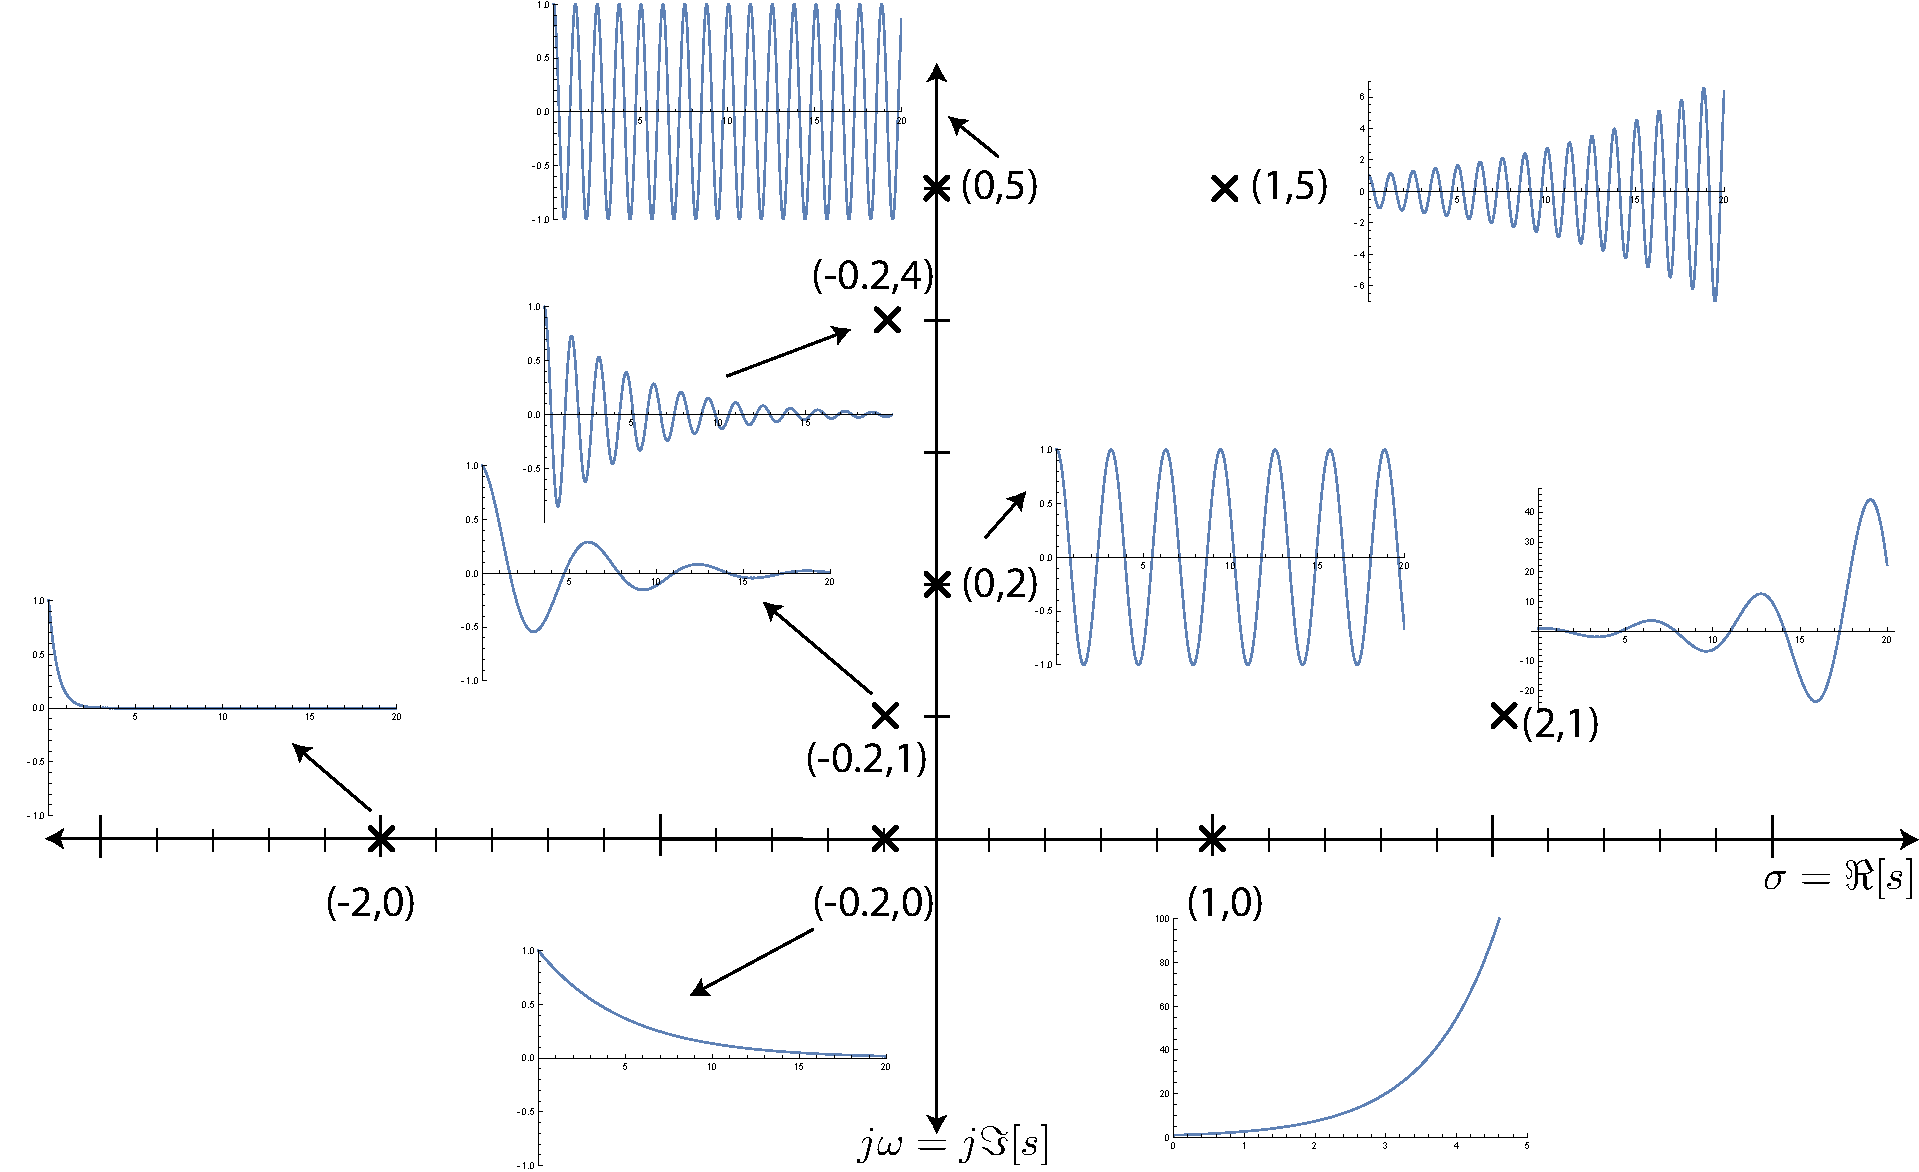
\includegraphics[width=.85\columnwidth]{exp_graph.pdf}
\caption{On the complex plane, the location of the argument $s$ to $e^{st}$ corresponds to either sinusoidal harmonic oscillation (on the imaginary axis), or exponential growth or decay (on the real axis).  Other off-axis locations are a combination of decaying or growing exponential sinusoidal waveforms.}
\label{fig:splane}
\end{figure}
%%%%%%%%%%%%%%%%%%%%%%%%%%%%%%%%%%%%%%%%%%%%%%%%%%%%%%%%%%%%%%%%%%%%%%%%%%%%%%%%%%%%%%%%
%%%%%%%%%%%%%%%%%%%%%%%%%%%%%%%%%%%%%%%%%%%%%%%%%%%%%%%%%%%%%%%%%%%%%%%%%%%%%%%%%%%%%%%%
%                                   SECTION 1.7                                        %
%%%%%%%%%%%%%%%%%%%%%%%%%%%%%%%%%%%%%%%%%%%%%%%%%%%%%%%%%%%%%%%%%%%%%%%%%%%%%%%%%%%%%%%%
%%%%%%%%%%%%%%%%%%%%%%%%%%%%%%%%%%%%%%%%%%%%%%%%%%%%%%%%%%%%%%%%%%%%%%%%%%%%%%%%%%%%%%%%
\section{Time Domain Characterization of Linear Systems}
%%%%%%%%%%%%%%%%%%%%%%%%%%%%%%%%%%%%%%%%%%%%
%             SUBSECTION 1.7.1             %
%%%%%%%%%%%%%%%%%%%%%%%%%%%%%%%%%%%%%%%%%%%%
\subsection{Unit Area Rectangular Function}
%%%%%%%%%%%%%%%%%%%%%%%%%%%%%%%%%%%%%%%%%%%%
%                 FIGURE                   %
%%%%%%%%%%%%%%%%%%%%%%%%%%%%%%%%%%%%%%%%%%%%
\begin{figure}[tb]
\centering
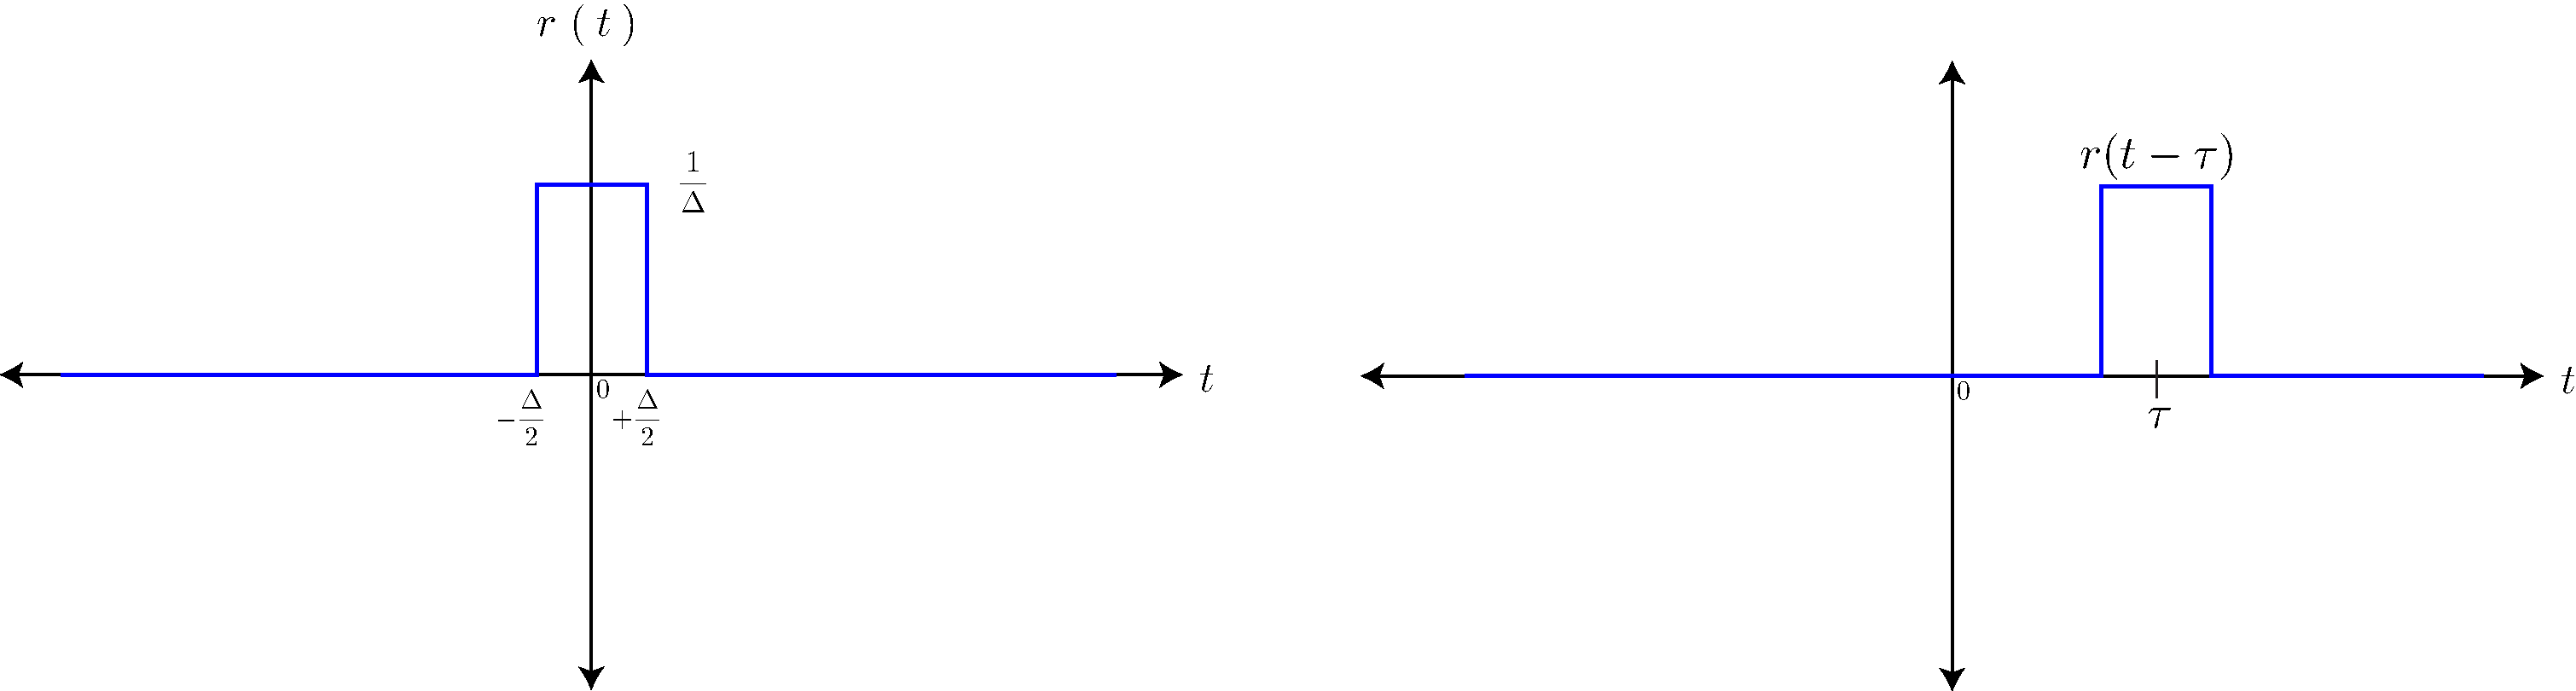
\includegraphics[width=1\columnwidth]{rect_func}
\caption{The unit rectangular function, centered at the origin or shifted by $\tau$. }
\label{fig:fun_rect}
\end{figure}
%%%%%%%%%%%%%%%%%%%%%%%%%%%%%%%%%%%%%%%%%%%%
A very convenient function, the \textbf{unit rectangular function}\index{Unit rectangular function}, shown in \emph{Fig.~\ref{fig:fun_rect}}, is defined as follows.  Consider a rectangular function with unit area:
    \begin{equation}
        r(t) = \left\{ 
        \begin{array}{cc} 
        \frac{1}{\Delta} & -\Delta/2 < t < \Delta/2 \\ 
        0  & \mathrm{otherwise} 
        \end{array} \right.
    \end{equation}
 By definition, we have a unit area function
    \begin{equation}
        \int_{-\infty}^{\infty} r(t) dt = 1
    \end{equation}
%%%%%%%%%%%%%%%%%%%%%%%%%%%%%%%%%%%%%%%%%%%%
%              SUB-SUBSECTION              %
%%%%%%%%%%%%%%%%%%%%%%%%%%%%%%%%%%%%%%%%%%%%
\subsubsection{Function Approximation}
As shown in \emph{Fig. ~\ref{fig:func_rect}}, we can approximate any function as a sum of rectangular shifted functions
    \begin{equation}
        x(t) \approx \sum_i x(i\tau) r(t - i\tau) \Delta
    \end{equation}
 As the rectangles become smaller and smaller, the representation becomes more accurate
 The key question is what happens as we take the limit of a very small time step $\Delta$?
%%%%%%%%%%%%%%%%%%%%%%%%%%%%%%%%%%%%%%%%%%%%
%                 FIGURE                   %
%%%%%%%%%%%%%%%%%%%%%%%%%%%%%%%%%%%%%%%%%%%%
\begin{figure}[tb]
\centering
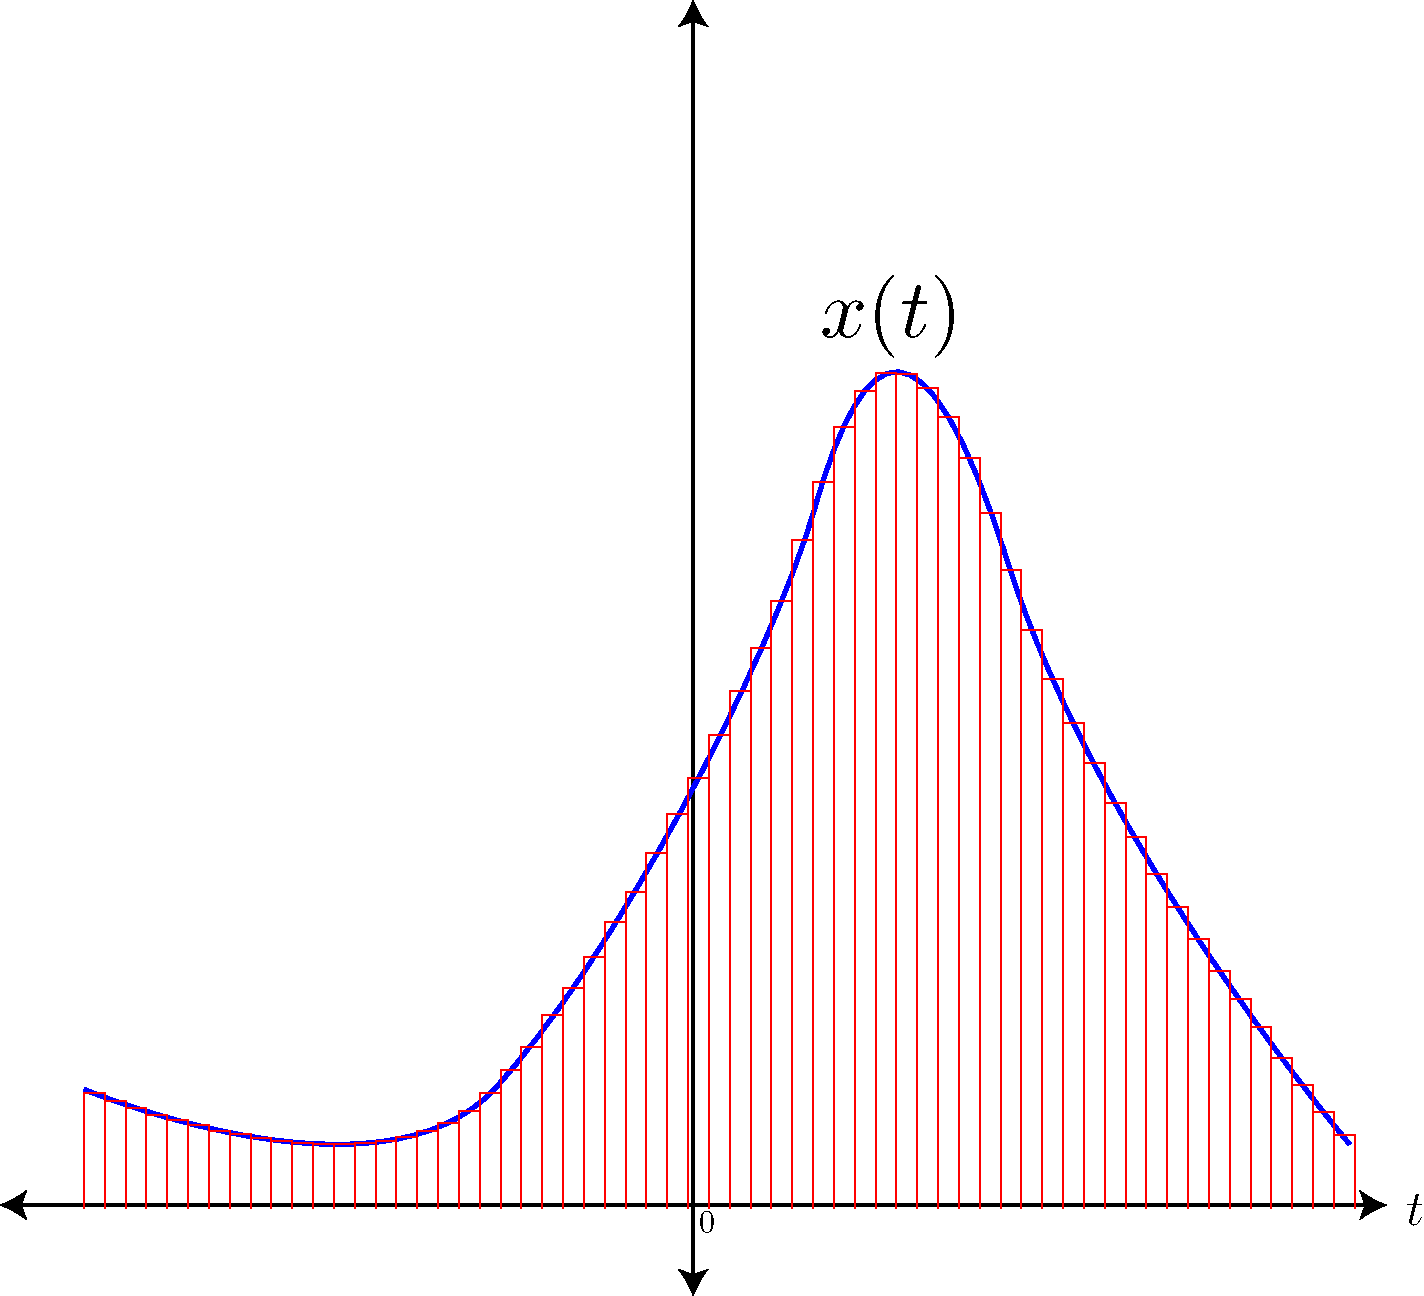
\includegraphics[width=.55\columnwidth]{func_rect}
\caption{Representation of a general function by a sum of shifted rectangular functions. }
\label{fig:func_rect}
\end{figure}
%%%%%%%%%%%%%%%%%%%%%%%%%%%%%%%%%%%%%%%%%%%%
%              SUB-SUBSECTION              %
%%%%%%%%%%%%%%%%%%%%%%%%%%%%%%%%%%%%%%%%%%%%
\subsubsection{The Delta Function $\delta(t)$ -- A Strange Beast}
%%%%%%%%%%%%%%%%%%%%%%%%%%%%%%%%%%%%%%%%%%%%
%                 FIGURE                   %
%%%%%%%%%%%%%%%%%%%%%%%%%%%%%%%%%%%%%%%%%%%%
\begin{figure}[tb]
\centering
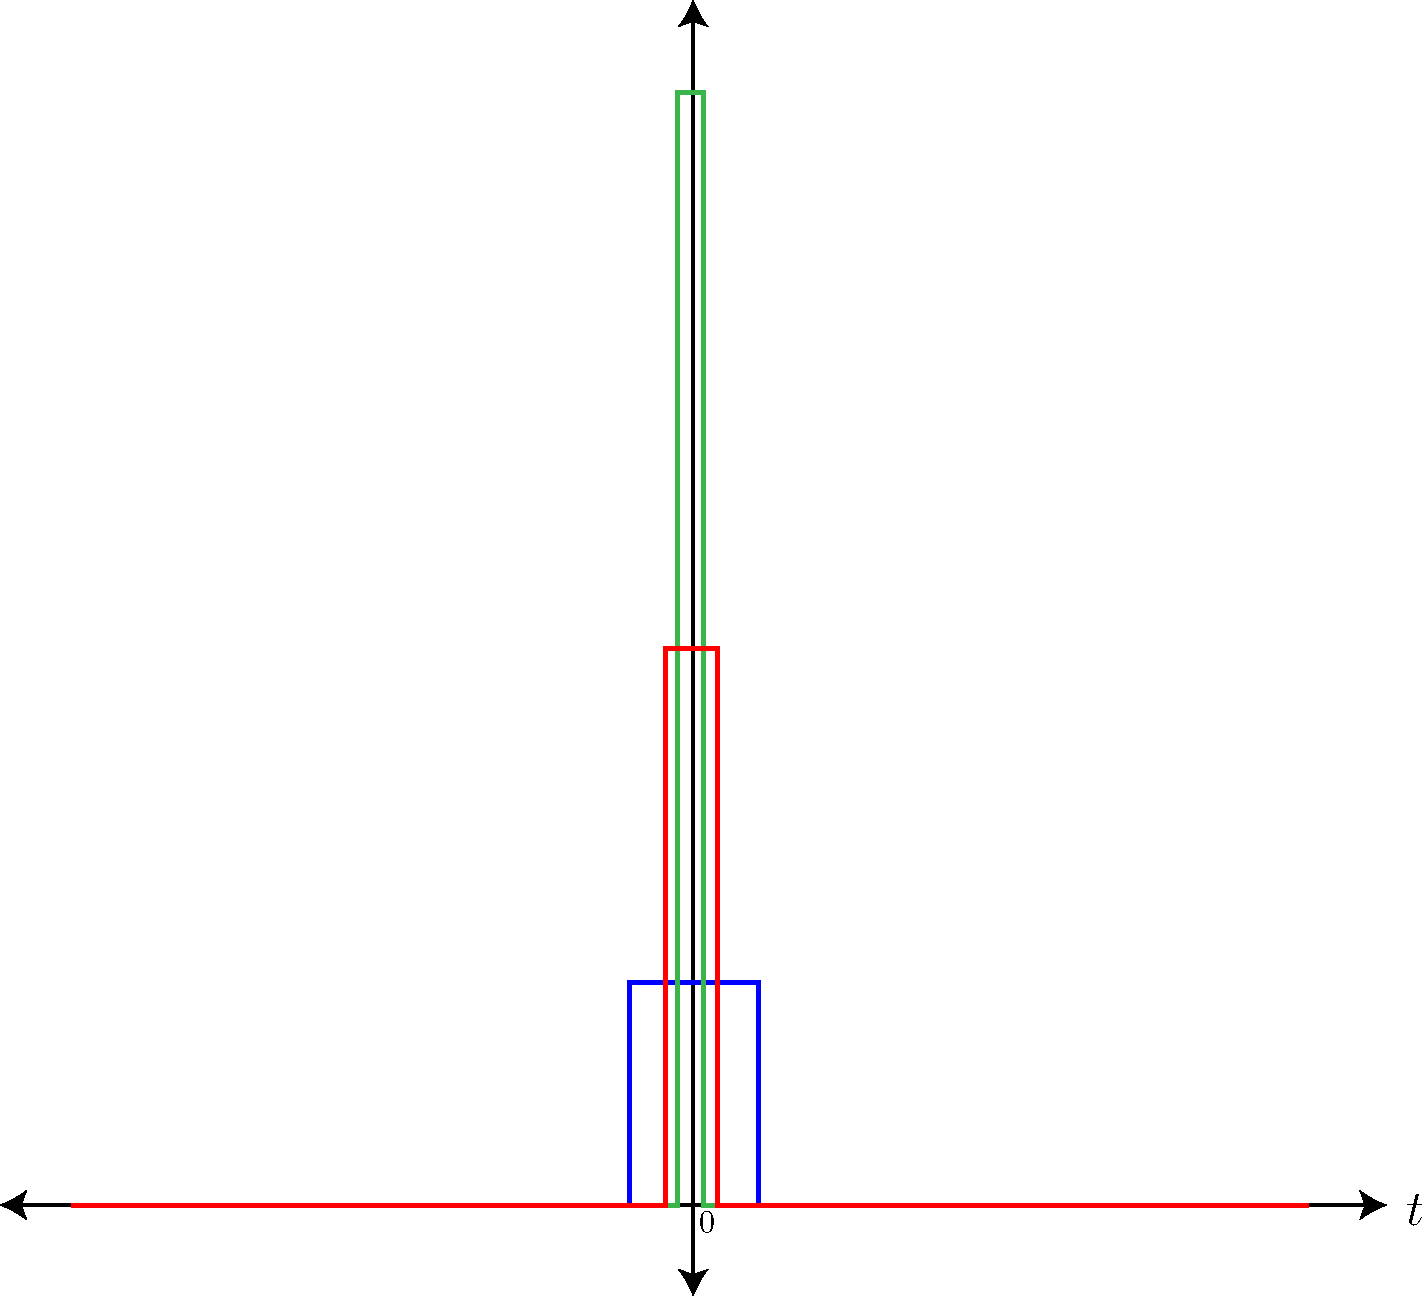
\includegraphics[width=.5\columnwidth]{rect_func_delta}
\caption{The "Delta Function" can be obtained through a limiting process by making the interval of the rectangular function shorter and shorter. }
\label{fig:rect_func_delta}
\end{figure}
%%%%%%%%%%%%%%%%%%%%%%%%%%%%%%%%%%%%%%%%%%%%
Now imagine taking the limit as $\Delta\rightarrow 0$
    \begin{equation}
        \lim_{\Delta\rightarrow0}{r\left(t\right)=\delta(t)}
    \end{equation}
What do we get?  Is this thing even a function?  A pictorial representation of the limiting process is shown in \emph{Fig.~\ref{fig:rect_func_delta}}.  We see that the function becomes more and more narrow and taller and taller.
%%%%%%%%%%%%%%%%%%%%%%%%%%%%%%%%%%%%%%%%%%%%
 No, it's not an ordinary function.\footnote{Mathematicians have made sense of it.  Now it's known as a distribution or generalized function.}  The \textbf{delta function}\index{Dirac Delta Function} was originally introduced by Oliver Heaviside $\sim$1900, Dirac co-invented it and gets credit as it's known as the "Dirac Delta Function".\footnote{Heaviside was derided by the mathematicians of the day for his methods.  He often got the right answer without being mathematically rigorous, but that's because he was way ahead of everyone in his techniques, and it took a while for the mathematical world to catch up.}
%%%%%%%%%%%%%%%%%%%%%%%%%%%%%%%%%%%%%%%%%%%%
%              SUB-SUBSECTION              %
%%%%%%%%%%%%%%%%%%%%%%%%%%%%%%%%%%%%%%%%%%%%
\subsubsection{Dirac Delta Sifting Property}
%%%%%%%%%%%%%%%%%%%%%%%%%%%%%%%%%%%%%%%%%%%%
%                 FIGURE                   %
%%%%%%%%%%%%%%%%%%%%%%%%%%%%%%%%%%%%%%%%%%%%
\begin{figure}[tb]
\centering
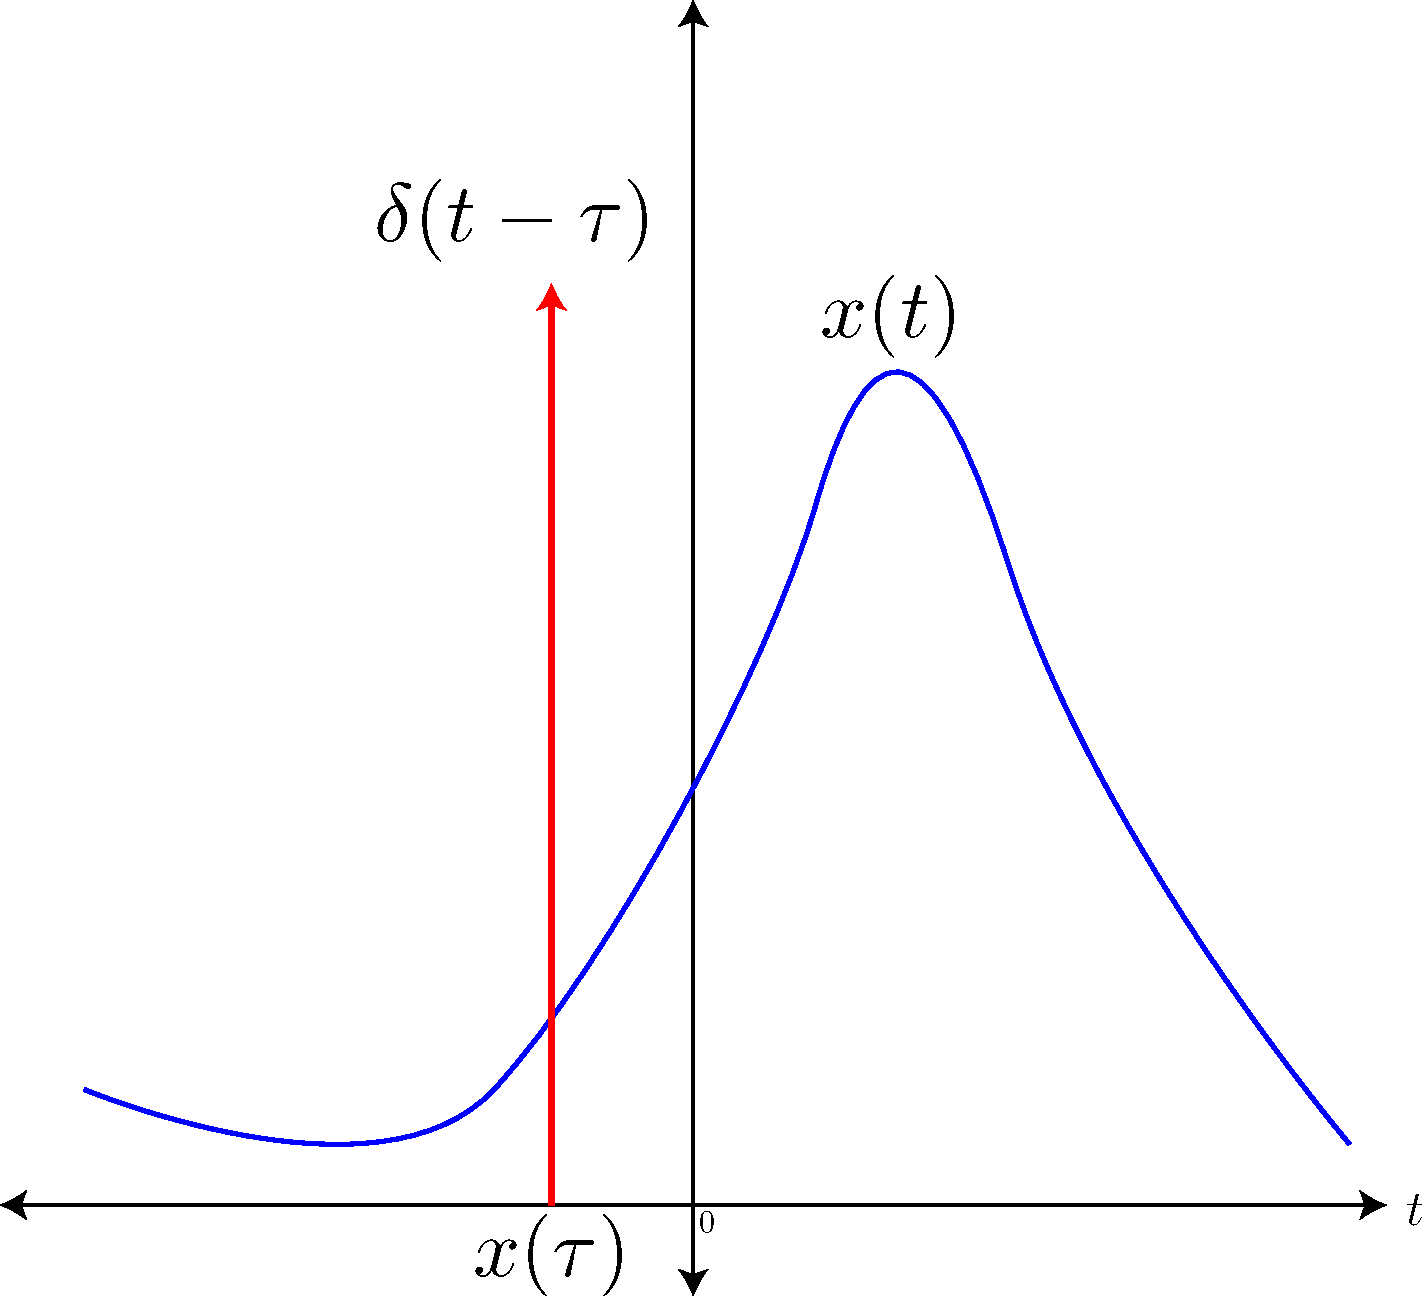
\includegraphics[width=.5\columnwidth]{delta_sift}
\caption{The \textbf{"sifting" property}\index{Dirac Delta Function!sifting property} of the Delta function yields the function value at any point. }
\label{fig:delta_sift}
\end{figure}
%%%%%%%%%%%%%%%%%%%%%%%%%%%%%%%%%%%%%%%%%%%%
As shown in \emph{Fig.~\ref{fig:delta_sift}}, one interesting thing about the Delta function is that it can be used to basically pick out a certain value of a function (because it's zero except at one location):
    \begin{equation}
        x\left(\tau\right)=\int\delta\left(t-\tau\right)x\left(t\right)dt
    \end{equation}
This is not obvious unless you take the limit and then it becomes clear that the integral converges to the value of the function.  So the Dirac Delta function is better defined in terms of this property, and many functions satisfy this function and can be used to define the Delta function.

Recall that we started by using the rectangular function to approximate any arbitrary function.  As we take the limit, we are reconstructing our function point-by-point using weighted sums of Delta functions.  To see this, simply start with the approximated  function as before
    \begin{equation}
        x(t) \approx \sum_i x(i\tau) r(t - i\tau) \Delta
    \end{equation}
As we take the limit, we expect that our approximation becomes more exact and we have the following integral:
    \begin{equation}
        x\left(t\right)=\int x\left(\tau\right)\delta\left(t-\tau\right)d\tau
    \end{equation}
In some ways this is not really a deep result in the sense of  saying that a function is a continuous stream of real numbers, and any particular value can be "sifted" out by multiplying by a delta and integrating around the delta.  If you think of the function as a vector, the delta function is like the vector $e_n = [0 \cdots 0\, 1\, 0 \cdots 0 ]^T$ with the $1$ in the n'th position. 
%%%%%%%%%%%%%%%%%%%%%%%%%%%%%%%%%%%%%%%%%%%%%%%%%%%%%%%%%%%%%%%%%%%%%%%%%%%%%%%%%%%%%%%%
%%%%%%%%%%%%%%%%%%%%%%%%%%%%%%%%%%%%%%%%%%%%%%%%%%%%%%%%%%%%%%%%%%%%%%%%%%%%%%%%%%%%%%%%
%                                   SECTION 1.8                                        %
%%%%%%%%%%%%%%%%%%%%%%%%%%%%%%%%%%%%%%%%%%%%%%%%%%%%%%%%%%%%%%%%%%%%%%%%%%%%%%%%%%%%%%%%
%%%%%%%%%%%%%%%%%%%%%%%%%%%%%%%%%%%%%%%%%%%%%%%%%%%%%%%%%%%%%%%%%%%%%%%%%%%%%%%%%%%%%%%%
\section{Back to Time Domain:  Impulse Response}
Up to now we studied the sinusoidal steady-state response using the complex exponential.  But we are now armed with the right tools to tackle the \textbf{general response}\index{Linear system!general response} of a linear system to an arbitrary input in time.  Using the fundamental properties of linearity and superposition, we have
    \begin{equation}
        y\left(t\right)=\ \mathbf{L}\left[x\left(t\right)\right]=\mathbf{L}\left[\int\delta\left(t-\tau\right)x\left(\tau\right)d\tau\right]
    \end{equation}
    \begin{equation}
        y\left(t\right)=\ \mathbf{L}\left[x\left(t\right)\right]=\int \mathbf{L}\left[\delta\left(t-\tau\right)x\left(\tau\right)\right]d\tau= \int x\left(\tau\right)\mathbf{L}\left[\delta\left(t-\tau\right)\right]d\tau
    \end{equation}
Let's define the impulse function as the response of a linear system to a Delta function applied at time $\tau$
    \begin{equation}
        h(t,\tau) \equiv  \mathbf{L}[\delta(t-\tau)]
    \end{equation}
Notice that in a time-invariant system, it should not matter when we apply the Delta function, as long as we shift the output.  So if $h(t)$ is the response to a Delta function at time 0, $h(t-\tau)$ is the response to an input applied at time $\tau$.  So in summary, for a linear time-invariant system (LTI), we only need to characterize the system response to a Delta function once and for all to find
    \begin{equation}
        h(t) \equiv  \mathbf{L}[\delta(t)]
    \end{equation}
This means that $h(t)$ contains all the information about the linear system. If we call the Dirac Delta function an "impulse", then for obvious reasons, we call $h(t)$ the \textbf{"impulse response function"}\index{Impulse response function}. 
%%%%%%%%%%%%%%%%%%%%%%%%%%%%%%%%%%%%%%%%%%%%
%             SUBSECTION 1.8.1             %
%%%%%%%%%%%%%%%%%%%%%%%%%%%%%%%%%%%%%%%%%%%%
\subsection{Convolution Operation}
We have demonstrated that any linear system input/output response can be represented by the following integral\index{Convolutions!integral}:
    \begin{equation}
        y(t) = \int_{-\infty}^{\infty} h(t-\tau) x(\tau) d\tau 
    \end{equation}
Think of this as the sum of the input weighted by the impulse response function.  The operation is known as the convolution operation and symbolically defined by the operator "$*$":  
    \begin{equation}
        y(t) = h(t) * x(t)
    \end{equation}
The symbol $*$ is the \textbf{convolution operator}\index{Convolutions!operator}. You can also change variables $x = t - \tau$ and write it as:
    \begin{equation}
        y(t) = \int_{\infty}^{-\infty} h(x) x(t-x) (-dx) = \int_{-\infty}^{\infty} h(x) x(t-x) dx 
    \end{equation}
In this equation, $x$ is just a dummy variable.  We can substitute $\tau$ to make the equation look the same as before (recall from calculus that  $\int_b^a x = -\int_a^b x$):
    \begin{equation}
        y(t) =  \int_{-\infty}^{\infty} x(t-\tau) h(\tau) d\tau
    \end{equation}
%%%%%%%%%%%%%%%%%%%%%%%%%%%%%%%%%%%%%%%%%%%%
%              SUB-SUBSECTION              %
%%%%%%%%%%%%%%%%%%%%%%%%%%%%%%%%%%%%%%%%%%%%
\subsubsection{Convolution Visualization}
%%%%%%%%%%%%%%%%%%%%%%%%%%%%%%%%%%%%%%%%%%%%
%                 FIGURE                   %
%%%%%%%%%%%%%%%%%%%%%%%%%%%%%%%%%%%%%%%%%%%%
\begin{figure}[tb]
\centering
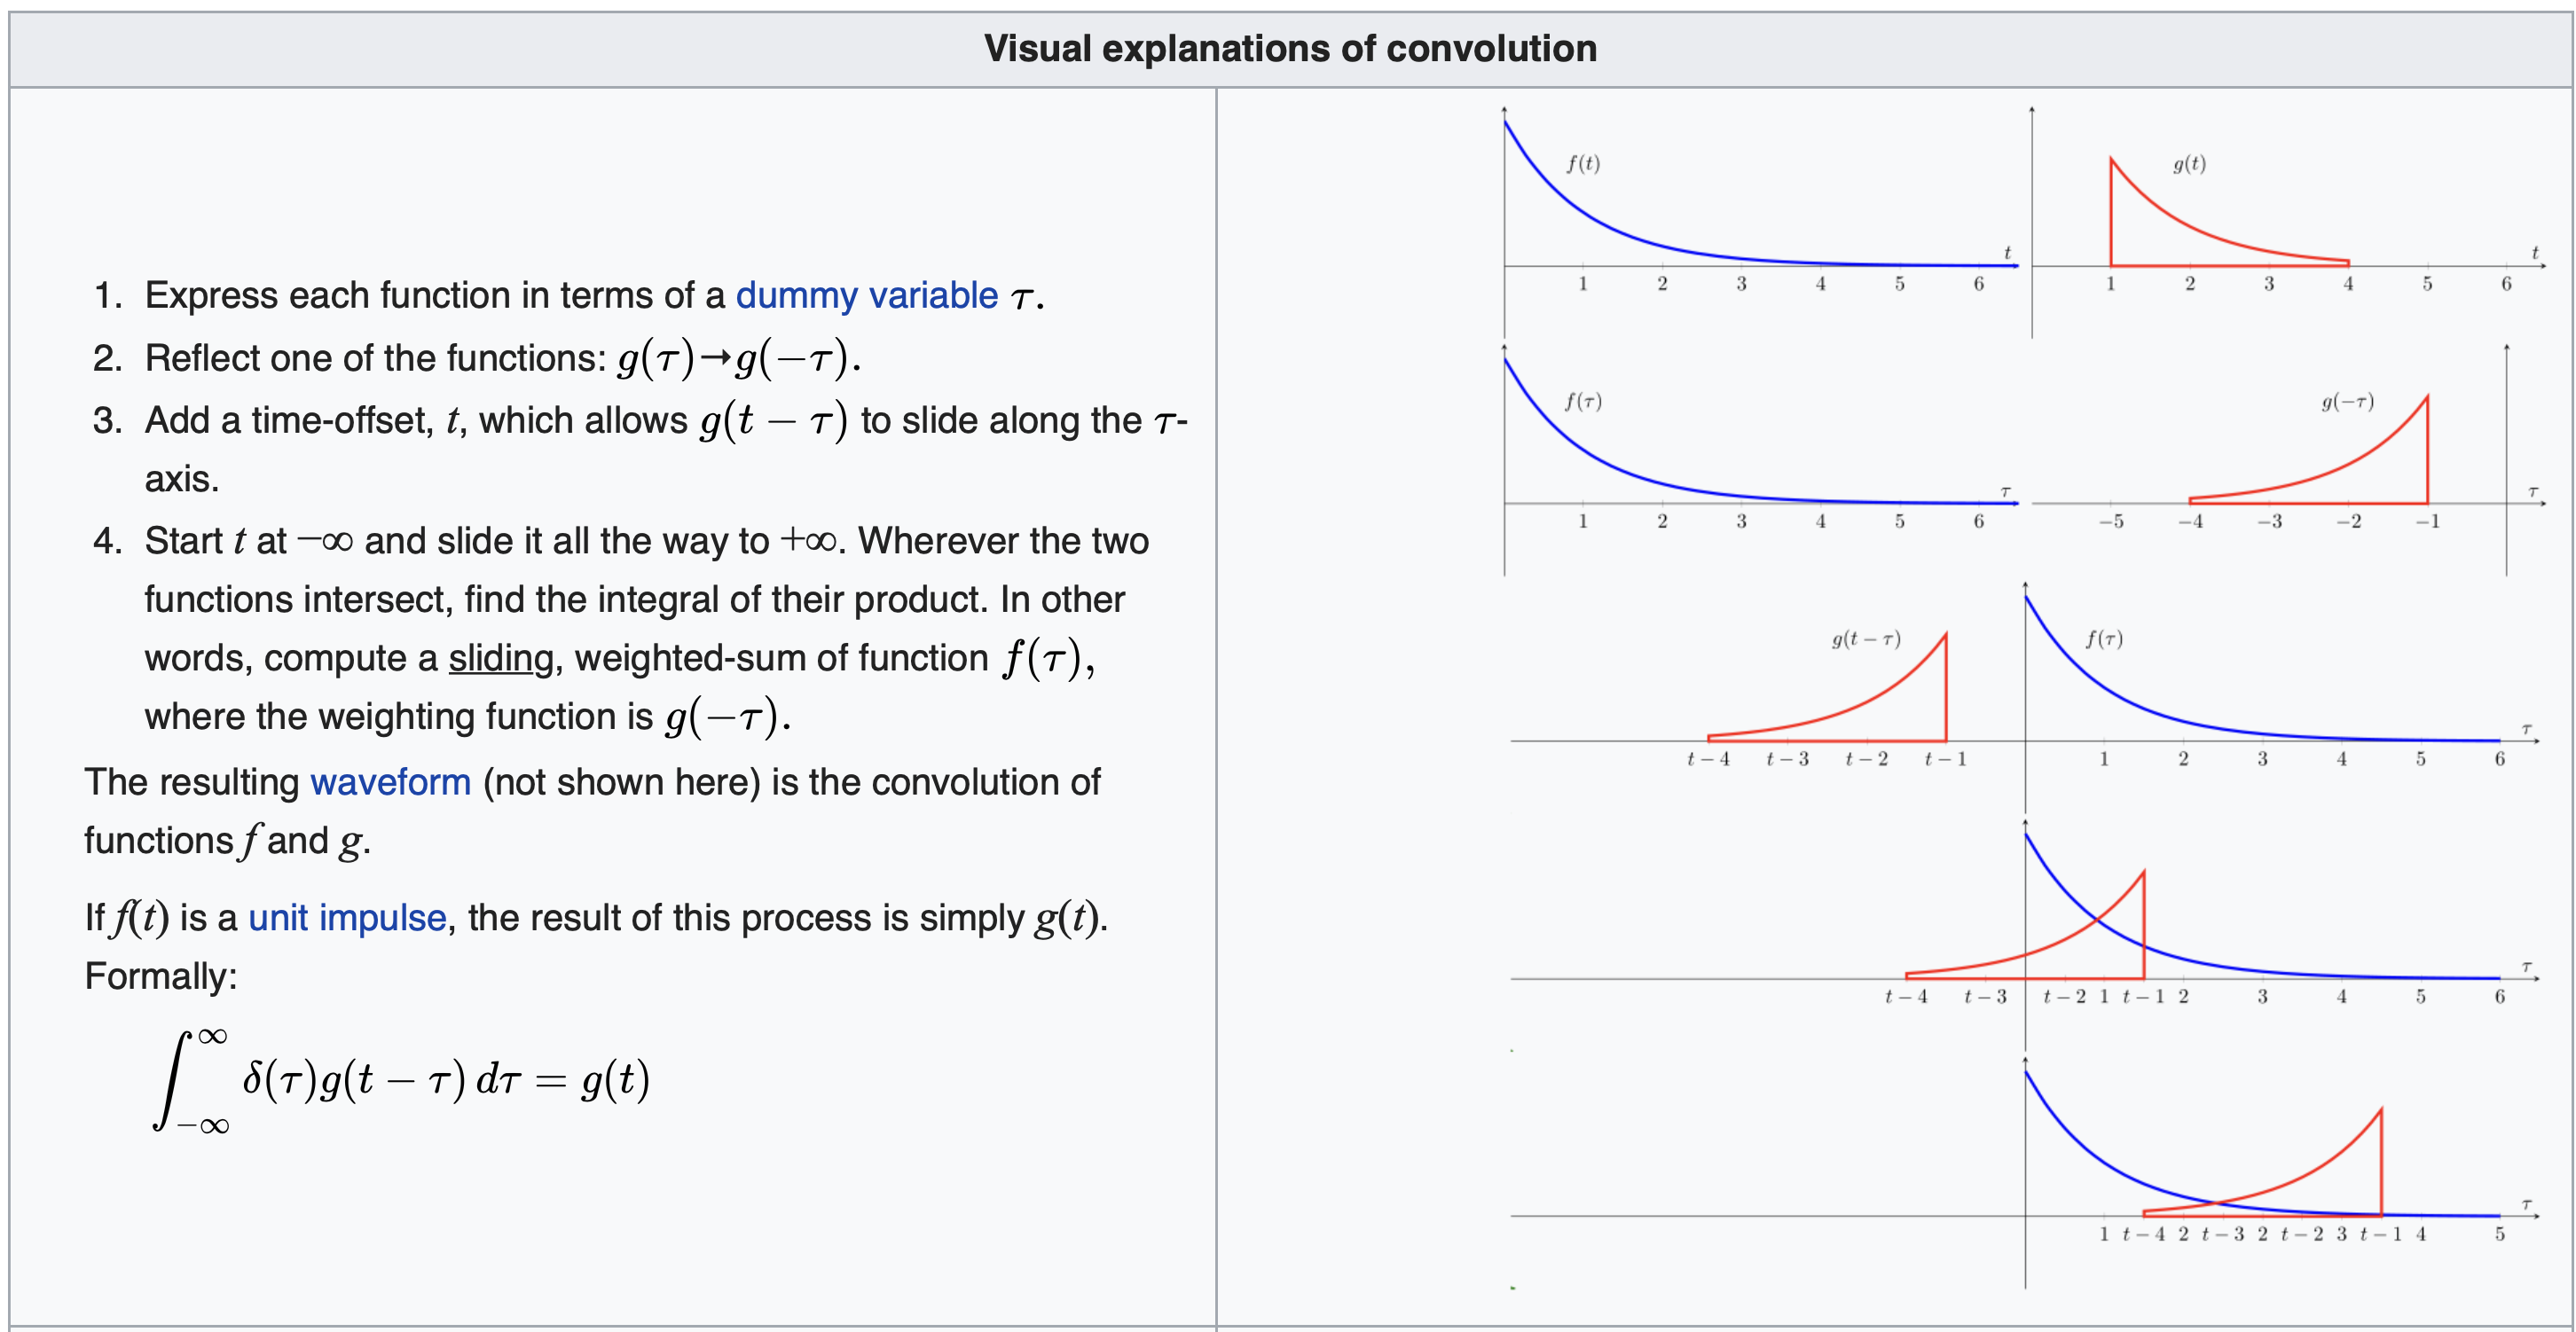
\includegraphics[width=.95\columnwidth]{conv_picture.png} 
\caption{The convolution operation visualized.  See Wikipedia for full details and an animation.}
\label{fig:conv_visual}
\end{figure}
%%%%%%%%%%%%%%%%%%%%%%%%%%%%%%%%%%%%%%%%%%%%
It's useful to visualize the convolution operation.  Note that the convolution operation takes in two functions and produces a new function.  The operation is described nicely on Wikipedia\footnote{\url{https://en.wikipedia.org/wiki/Convolution}} reproduced here in \emph{Fig.~\ref{fig:conv_visual}}.  As described in the figure, we first express each function in terms of the dummy variable (of integration) $\tau$.  Next, we reflect one of the functions about the time axis.  For example, $h(\tau)$ becomes $h(-\tau)$.  The physical explanation for this will be described shortly.  Next we compute a sliding weighted-sum of the function $x(\tau)$ with $h(t-\tau)$.  Only points where the two functions intersect contribute significantly to the waveform.  
%%%%%%%%%%%%%%%%%%%%%%%%%%%%%%%%%%%%%%%%%%%%
%              SUB-SUBSECTION              %
%%%%%%%%%%%%%%%%%%%%%%%%%%%%%%%%%%%%%%%%%%%%
\subsubsection{Memory}
%%%%%%%%%%%%%%%%%%%%%%%%%%%%%%%%%%%%%%%%%%%%
%                 FIGURE                   %
%%%%%%%%%%%%%%%%%%%%%%%%%%%%%%%%%%%%%%%%%%%%
\begin{figure}[tb]
\begin{tabular}{cc}
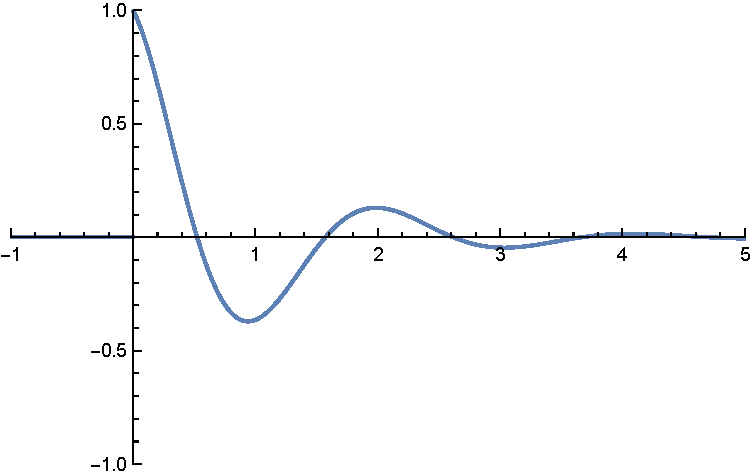
\includegraphics[width=.4\columnwidth]{impulse1_long.pdf} &
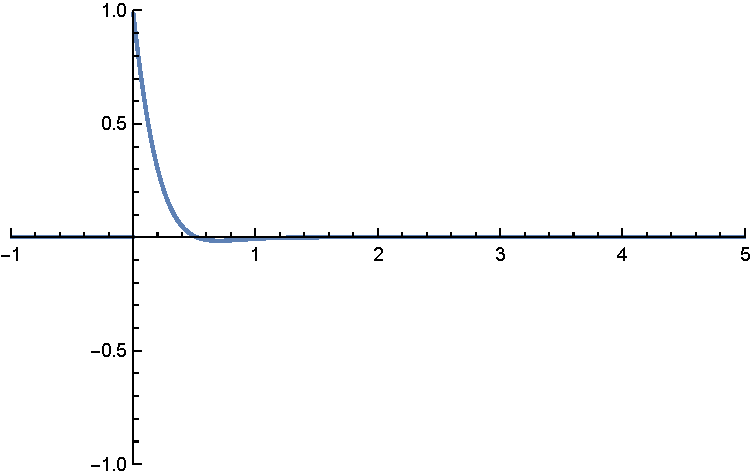
\includegraphics[width=.4\columnwidth]{impulse2_short.pdf} \\
\end{tabular}
\caption{Two hypothetical impulse response functions are shown.  One is long and oscillates, the second is short and delays exponentially.}
\label{fig:memory}
\end{figure}
%%%%%%%%%%%%%%%%%%%%%%%%%%%%%%%%%%%%%%%%%%%%
For example, if $h(t)$ is mostly zero except over a small interval, 
%%%%%%%%%%%%%%%%%%%%%%%%%%%%%%%%%%%%%%%%%%%%
The fact that the impulse response function has time duration is an indication that the system has memory.  The current output depends not only on the current input, but also past values of the input.  The longer the duration of the impulse response function, the more "memory" the system has.  Capacitors and inductors store energy and act as memory in circuits.  They store energy in the magnetic and electric fields, and resonance can occur because these forms of energy can be exchanged.  The impulse response function for a system with no memory is just another delta function!  Two examples are shown in \emph{Fig.~\ref{fig:memory}} to illustrate a system with a longer vacillating impulse response versus a system that has a short and exponentially decaying impulse response.  

This should help you understand why we needed to flip the impulse response in the convolution operation (or equivalently the input function).  Notice first that the impulse function is necessarily zero until time zero. This is because the system is causal and there can be no output if there's no input.  Next, notice that by flipping the impulse response and taking a sliding weighted sum with the input, we're including the contribution of past inputs on the current input.  If the impulse response is short and decaying exponentially, then only a small amount of past inputs influence the current input.  On the other hand, if the impulse response is longer, then the system remembers the history of the input for a longer duration and we must include those terms to figure out the current output.
%%%%%%%%%%%%%%%%%%%%%%%%%%%%%%%%%%%%%%%%%%%%
%              SUB-SUBSECTION              %
%%%%%%%%%%%%%%%%%%%%%%%%%%%%%%%%%%%%%%%%%%%%
\subsubsection{The Delta Function "Hammer":  Mechanical Analogy}
%%%%%%%%%%%%%%%%%%%%%%%%%%%%%%%%%%%%%%%%%%%%
%                 FIGURE                   %
%%%%%%%%%%%%%%%%%%%%%%%%%%%%%%%%%%%%%%%%%%%%
\begin{figure}[tb]
\centering
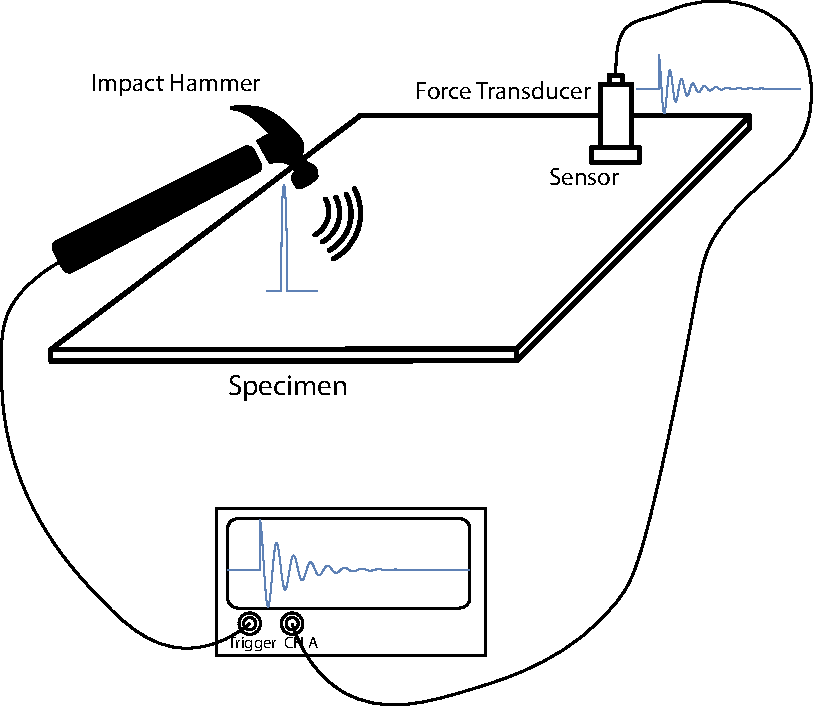
\includegraphics[width=.5\columnwidth]{hammer_resonance}
\caption{A measurement setup to record the impulse response of a mechanical system. }
\label{fig:hammer_setup}
\end{figure}
%%%%%%%%%%%%%%%%%%%%%%%%%%%%%%%%%%%%%%%%%%%%
Another way to look at a delta function is to think of it like hitting your system with a hammer (see \emph{Fig.~\ref{fig:hammer_setup}}).  It is an impulsive input that excites the system.  After such an excitation, the system will "vibrate" in its natural modes and these vibrations will eventually die out.  The time that the vibrations last is related to the depth of the system's memory.  The vibrations are related to the fact that the system can store kinetic and potential energy and these modes complement each other.  Loss in the system causes this stored energy to eventually dissipate.  In fact, one way to measure the impulse response is exactly with the setup shown.  The hammer is implemented an electromechanical solenoid, and the actuation signal is fed to the trigger of the oscilloscope (or other recording device).  The vibrations are picked up by a force transducer and carefully recorded, yielding the impulse response.     
%%%%%%%%%%%%%%%%%%%%%%%%%%%%%%%%%%%%%%%%%%%%%%%%%%%%%%%%%%%%%%%%%%%%%%%%%%%%%%%%%%%%%%%%
%%%%%%%%%%%%%%%%%%%%%%%%%%%%%%%%%%%%%%%%%%%%%%%%%%%%%%%%%%%%%%%%%%%%%%%%%%%%%%%%%%%%%%%%
%                                   SECTION 1.9                                        %
%%%%%%%%%%%%%%%%%%%%%%%%%%%%%%%%%%%%%%%%%%%%%%%%%%%%%%%%%%%%%%%%%%%%%%%%%%%%%%%%%%%%%%%%
%%%%%%%%%%%%%%%%%%%%%%%%%%%%%%%%%%%%%%%%%%%%%%%%%%%%%%%%%%%%%%%%%%%%%%%%%%%%%%%%%%%%%%%%
\section{Step and Pulse Response}
%%%%%%%%%%%%%%%%%%%%%%%%%%%%%%%%%%%%%%%%%%%%
%                 FIGURE                   %
%%%%%%%%%%%%%%%%%%%%%%%%%%%%%%%%%%%%%%%%%%%%
\begin{figure}[tb]
\centering
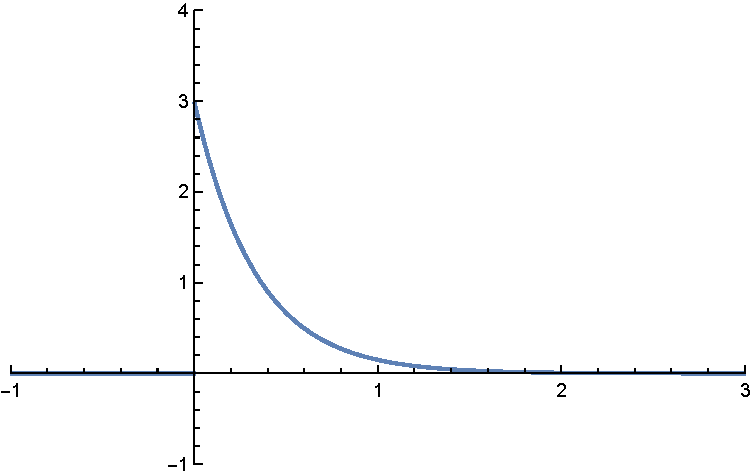
\includegraphics[width=.6\columnwidth]{impulse_resp}
\caption{The impulse response for the low-pass filtered analyzed earlier in the frequency domain. }
\label{fig:impulse_resp}
\end{figure}
%%%%%%%%%%%%%%%%%%%%%%%%%%%%%%%%%%%%%%%%%%%%
Consider a system with an impulse response shown in \emph{Fig.~\ref{fig:impulse_resp}}.  This is in fact the impulse response function for a low-pass filter:\footnote{See tables~\ref{fig:laplace_table} and~\ref{fig:laplace_xform} of transforms later in this lecture.}
    \begin{equation}
        h(t) = u(t) \frac{1}{\tau} e^{-t/\tau}
    \end{equation}
Notice that the system has a time constant $\tau = RC$ that corresponds to the amount of time the system responds to an impulse input ($\tau = 1/3$).  Here $u(t)$ is the step function (zero until time zero, and then unity thereafter).  As discussed earlier, the impulse response is necessarily zero until time zero, and the $u(t)$ enforces this condition.  If you now imagine an arbitrary input, each time point is a weighted sum of the current input and past inputs, with an exponentially decaying amplitude for past inputs.  Only the recent $\sim \tau$ inputs really make an impact, and earlier inputs are "forgotten".  
%%%%%%%%%%%%%%%%%%%%%%%%%%%%%%%%%%%%%%%%%%%%
%                 FIGURE                   %
%%%%%%%%%%%%%%%%%%%%%%%%%%%%%%%%%%%%%%%%%%%%
\begin{figure}[tb]
\centering
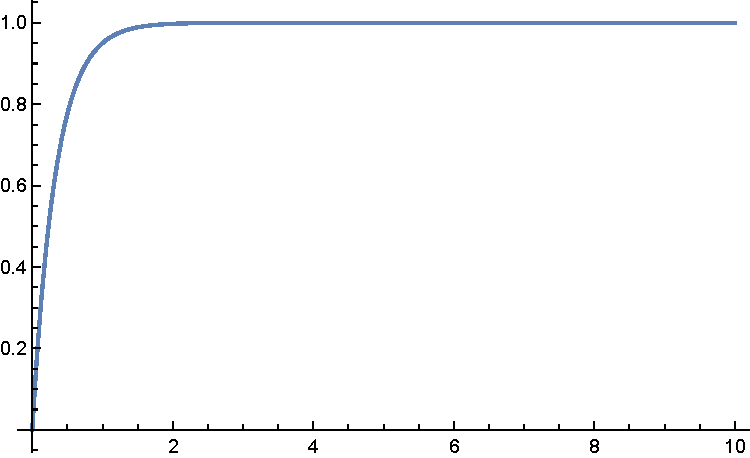
\includegraphics[width=.5\columnwidth]{step_resp}
\caption{The step response of a low-pass filter. }
\label{fig:step_resp}
\end{figure}
%%%%%%%%%%%%%%%%%%%%%%%%%%%%%%%%%%%%%%%%%%%%
%             SUBSECTION 1.9.1             %
%%%%%%%%%%%%%%%%%%%%%%%%%%%%%%%%%%%%%%%%%%%%
\subsection{Step Response}
A very interesting input is the \textbf{"step input"}\index{Step input}\index{Step response}, or application of $u(t)$ to our system.  From what we know, we can calculate the response to a step by using a convolution:
    \begin{equation}
        y(t) = h(t) * u(t) = \left( 1 - e^{-3 t} \right) u(t) 
    \end{equation}
The response is plotted in \emph{Fig.~\ref{fig:step_resp}}. The step has a very sharp transition at the input, but at the output it's smoothed out because each output point is an average of the current input and past inputs.  Since at the moment of the transition, all past inputs are zero, the output cannot track the input instantaneously.
\newpage
%%%%%%%%%%%%%%%%%%%%%%%%%%%%%%%%%%%%%%%%%%%%
%             SUBSECTION 1.9.2             %
%%%%%%%%%%%%%%%%%%%%%%%%%%%%%%%%%%%%%%%%%%%%
\subsection{Sinusoidal Response}
%%%%%%%%%%%%%%%%%%%%%%%%%%%%%%%%%%%%%%%%%%%%
%                 FIGURE                   %
%%%%%%%%%%%%%%%%%%%%%%%%%%%%%%%%%%%%%%%%%%%%
\begin{figure}[tb]
\centering
\begin{tabular}{cc}
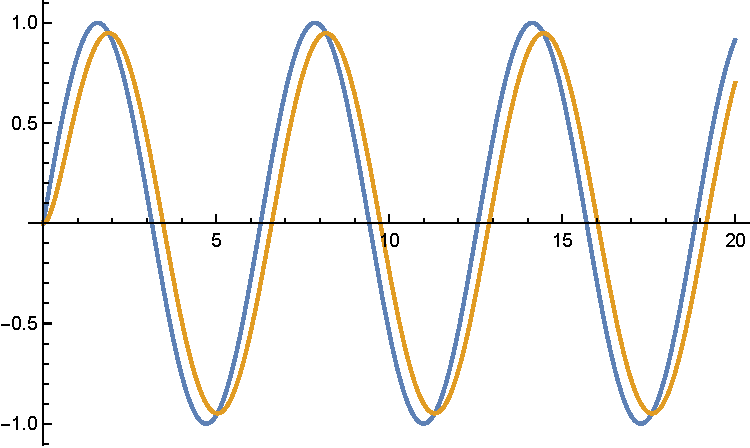
\includegraphics[width=.45\columnwidth]{slow_sine.pdf} &
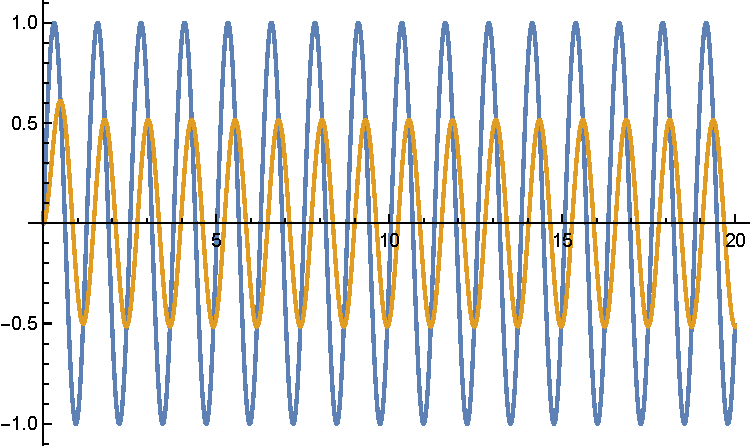
\includegraphics[width=.45\columnwidth]{fast_sine.pdf} \\
\end{tabular}
\caption{The response of a linear system to a "slow" and "fast" sinusoid.  Slow means the period of oscillation is smaller than the filter characteristic time constant $\tau$.  Fast means the opposite.}
\label{fig:fast_slow_resp}
\end{figure}
%%%%%%%%%%%%%%%%%%%%%%%%%%%%%%%%%%%%%%%%%%%%
As shown in \emph{Fig.~\ref{fig:fast_slow_resp}}, if the input changes slower than the time scale of $\tau$, or if the frequency of the input is lower than roughly $1/\tau$, then the output is a smoothed version of the input (each time point is blurred by the width of the impulse response).  Fast transitions are smoothed out and don't appear at the output.   If the input changes very quickly, several cycles of the input are averaged out and produce only a small output.  This is how the filter works as high frequency signals are attenuated by the low-pass filter.  If the oscillation frequency is very slow with respect to $\tau$, the impulse response "looks like" a delta function with no memory and just passes the current input to the output.
%%%%%%%%%%%%%%%%%%%%%%%%%%%%%%%%%%%%%%%%%%%%
%             SUBSECTION 1.9.2             %
%%%%%%%%%%%%%%%%%%%%%%%%%%%%%%%%%%%%%%%%%%%%
\subsection{Pulse Response}
%%%%%%%%%%%%%%%%%%%%%%%%%%%%%%%%%%%%%%%%%%%%
%                 FIGURE                   %
%%%%%%%%%%%%%%%%%%%%%%%%%%%%%%%%%%%%%%%%%%%%
\begin{figure}[tb]
\centering
\begin{tabular}{cc}
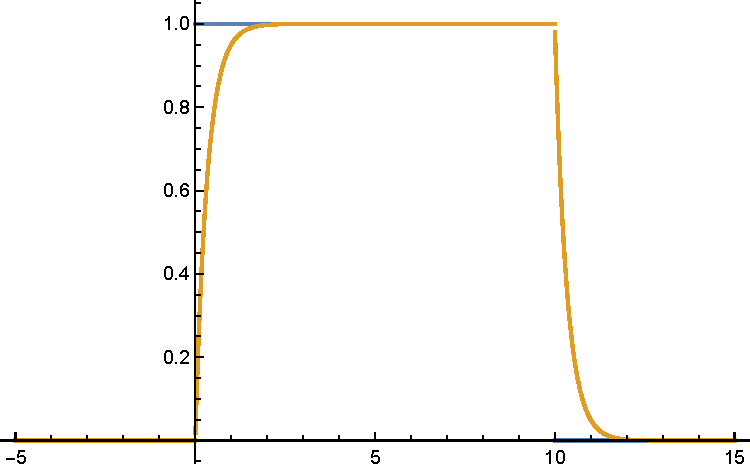
\includegraphics[width=.4\columnwidth]{long_pulse.pdf} &
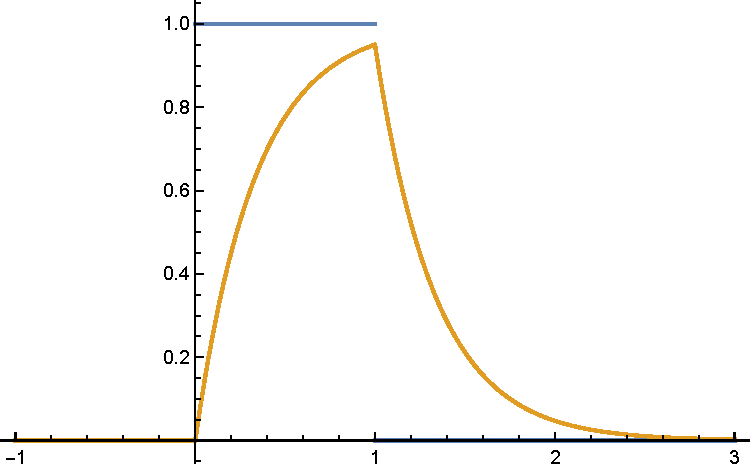
\includegraphics[width=.4\columnwidth]{fast_pulse.pdf} \\
\end{tabular}
\caption{The \textbf{pulse response}\index{Pulse response} of a low-pass filter.  Note that the shorter pulse has been expanded for clarity (see the time scale). }
\label{fig:pulse_resp}
\end{figure}
%%%%%%%%%%%%%%%%%%%%%%%%%%%%%%%%%%%%%%%%%%%%
Now let's see what happens to a pulse.  By superposition, this is just two unit-step responses, so we can easily reconstruct the response as shown in \emph{Fig.~\ref{fig:pulse_resp}}.  If the pulse is wide, then the output has enough time to settle and the output pulse is a faithful representation of the input.  If the pulse width is shorter than the time-constant of the filter, there is insufficient time for the output to settle, and the pulse is distorted.  In high speed communication systems, we need to ensure the system has enough \textbf{bandwidth}\index{Bandwidth} to allow the highest frequency pulses to get through.  
%%%%%%%%%%%%%%%%%%%%%%%%%%%%%%%%%%%%%%%%%%%%%%%%%%%%%%%%%%%%%%%%%%%%%%%%%%%%%%%%%%%%%%%%
%%%%%%%%%%%%%%%%%%%%%%%%%%%%%%%%%%%%%%%%%%%%%%%%%%%%%%%%%%%%%%%%%%%%%%%%%%%%%%%%%%%%%%%%
%                                   SECTION 1.10                                       %
%%%%%%%%%%%%%%%%%%%%%%%%%%%%%%%%%%%%%%%%%%%%%%%%%%%%%%%%%%%%%%%%%%%%%%%%%%%%%%%%%%%%%%%%
%%%%%%%%%%%%%%%%%%%%%%%%%%%%%%%%%%%%%%%%%%%%%%%%%%%%%%%%%%%%%%%%%%%%%%%%%%%%%%%%%%%%%%%%
\section{Frequency Domain Characterization of Linear Systems}
We started this chapter by discussion of the steady-state sinusoidal response of a linear system.  We found that we can use complex exponential inputs to quickly and efficiently calculate the output, and by sweeping the frequency, we obtain the \textbf{spectral response}\index{Spectral response} of the system $H(s)$ (the complex eigenvalues) that completely characterizes the system.   Next we find that in the time domain, the impulse response is a way to "probe" a linear system to determine its behavior.  In other words both $H(s)$ and $h(t)$ are a very special responses that characterizes the system.  One comes from the complex exponential input $e^{st}$ and the other from the the application of a delta function.  How are these functions $H(s)$ and $h(t)$ related?
%%%%%%%%%%%%%%%%%%%%%%%%%%%%%%%%%%%%%%%%%%%%
%             SUBSECTION 1.10.1            %
%%%%%%%%%%%%%%%%%%%%%%%%%%%%%%%%%%%%%%%%%%%%
\subsection{Relation to Complex Exponential}
Recall that we found that the complex exponential\index{Complex exponential} is an eigenfunction\index{Eigenfunction} for our linear system:
    \begin{equation}
        \mathbf{L} [ e^{st} ] = H(s) e^{st}
    \end{equation}
But that means that we can apply the convolution integral\index{Convolutions!integral} to the input $e^{st}$ and equate the two outputs:
    \begin{equation}
        \mathbf{L} [ e^{st} ] = H(s) e^{st}  = \int_{-\infty}^{\infty} h(t-\tau) e^{s\tau} d\tau
    \end{equation}
A simple manipulation shows that:
    \begin{align*}
        H(s) &= \int h(t-\tau) e^{s\tau} e^{-st} d\tau\\
        &= \int h(t-\tau) e^{-s(t- \tau)} d\tau\\
        &= \int_{\infty}^{-\infty} h(x) e^{-sx} (-dx) &\text{\emph{Let $x = t - \tau$}}
    \end{align*}
Thus, we have:
    \begin{equation}
        H(s) = \int_{-\infty}^{\infty} h(x) e^{-sx} dx
    \end{equation}
This equation shows us that $H(s)$ and $h(t)$ are indeed related in a very special way.
%%%%%%%%%%%%%%%%%%%%%%%%%%%%%%%%%%%%%%%%%%%%
%              SUB-SUBSECTION              %
%%%%%%%%%%%%%%%%%%%%%%%%%%%%%%%%%%%%%%%%%%%%
\subsubsection{Laplace Transform}
 We derived a very important relation between the transfer function and the impulse response which is known as the \textbf{Laplace Transform}\index{Laplace transform} $\mathcal{L}$:
    \begin{equation}
        H(s) = \int_{-\infty}^{\infty} h(t) e^{-st} dt = \mathcal{L} \left\{ h(t) \right\}
    \end{equation}
This can be interpreted as transforming a \textbf{time-domain}\index{Time-domain} function to the \textbf{"s-domain"}\index{S-domain}, which is the general complex \textbf{frequency-domain}\index{Frequency-domain}.  In this book we will not use Laplace Transforms explicitly, instead we will mostly use the transfer function in the frequency domain:  $H(j\omega)$, which is nothing but evaluating the transfer function $H(s)$ for $s=j\omega$.  
%%%%%%%%%%%%%%%%%%%%%%%%%%%%%%%%%%%%%%%%%%%%
Even though we won't make extensive use of the Laplace Transform, we nevertheless spent some time to highlight these important concepts and relations because they show a deep connection between the frequency domain response $H(j\omega)$ and the time domain response.
%%%%%%%%%%%%%%%%%%%%%%%%%%%%%%%%%%%%%%%%%%%%
%             SUBSECTION 1.10.2            %
%%%%%%%%%%%%%%%%%%%%%%%%%%%%%%%%%%%%%%%%%%%%
\subsection{De-convolving the Convolution}
In fact, one of the most important relations is how convolution in time translates to the frequency domain.  Consider the (complicated) convolution operator and take the results into the Laplace domain:
    \begin{equation}
        Y(s) = \mathcal{L} \left\{ x(t) * h(t) \right\} = \mathcal{L} \left\{  \int h(t-\tau) x(\tau) d\tau \right\} 
    \end{equation}
Use the definition of the Laplace Transform
    \begin{equation}
        Y(s) = \int \left( \int h(t-\tau) x(\tau) d\tau \right) e^{-s t} dt
    \end{equation}
Notice that if we make a simple change of notation and call $y = t-\tau$ the new dummy variable, we have:
    \begin{align*}
        Y(s) &= \int \int h(\underbrace{t-\tau}_{y}) x(\tau) e^{-s t} d\tau dt\\
        &= \int \int h(y) e^{-s(y + \tau)} x(\tau) dy d\tau &\text{\emph{$t = y + \tau$}}
    \end{align*}
Each integral is only a function of one variable, so we can separate them out:
    \begin{equation}
        Y(s) = \left( \int h(y) e^{-sy} dy \right) \left( \int x(\tau) e^{-s \tau} d\tau \right)
    \end{equation}
 Or more simply, the convolution is a (simple) product in the Laplace domain:
    \begin{equation}
        Y(s) = H(s) X(s) 
    \end{equation}
This is a very important result.  Not only is it more efficient to work directly in the \textbf{Laplace domain}\index{Laplace domain} (or frequency domain) when computing the response of a linear system, but it is also much easier to visualize what's going on.  A filter can be visualized very simply in the frequency domain. For an arbitrary input, if we compute it's Laplace (or Fourier, see below) Transform, we can find the output by simply multiplying the two and doing an inverse transform.  In many cases, we don't even need to do the inverse transform, which is not a very simple calculation to carry out.  We simply use the concept of frequency domain to better understand our system.
%%%%%%%%%%%%%%%%%%%%%%%%%%%%%%%%%%%%%%%%%%%%
%              SUB-SUBSECTION              %
%%%%%%%%%%%%%%%%%%%%%%%%%%%%%%%%%%%%%%%%%%%%
\subsubsection{Laplace Transform Properties}
The properties of the Laplace Transform are summarized in \emph{Fig.~\ref{fig:laplace_table}}.   Most are easily derived and are provided here just for reference.  We just proved the most important property related to the convolution.    
%%%%%%%%%%%%%%%%%%%%%%%%%%%%%%%%%%%%%%%%%%%%
%              SUB-SUBSECTION              %
%%%%%%%%%%%%%%%%%%%%%%%%%%%%%%%%%%%%%%%%%%%%
\subsubsection{Laplace Transform Table}
From Wikipedia\footnote{\url{https://en.wikipedia.org/wiki/Laplace_transform}}, the table in \emph{Fig.~\ref{fig:laplace_xform}} shows some common Laplace Transform "pairs", or the s-domain representation for some common functions.  This table is important because in practice we hardly ever evaluate the Laplace Transform integral, especially in the reverse direction.  Instead, the lookup table is used for common functions and special techniques, such as partial fraction expansions, can be used to put a rational function into standard form.  We showed earlier that most linear systems do in fact generate a rational function transfer function.
\newpage
%%%%%%%%%%%%%%%%%%%%%%%%%%%%%%%%%%%%%%%%%%%%
%                 FIGURE                   %
%%%%%%%%%%%%%%%%%%%%%%%%%%%%%%%%%%%%%%%%%%%%
\begin{figure}[tb]
\centering
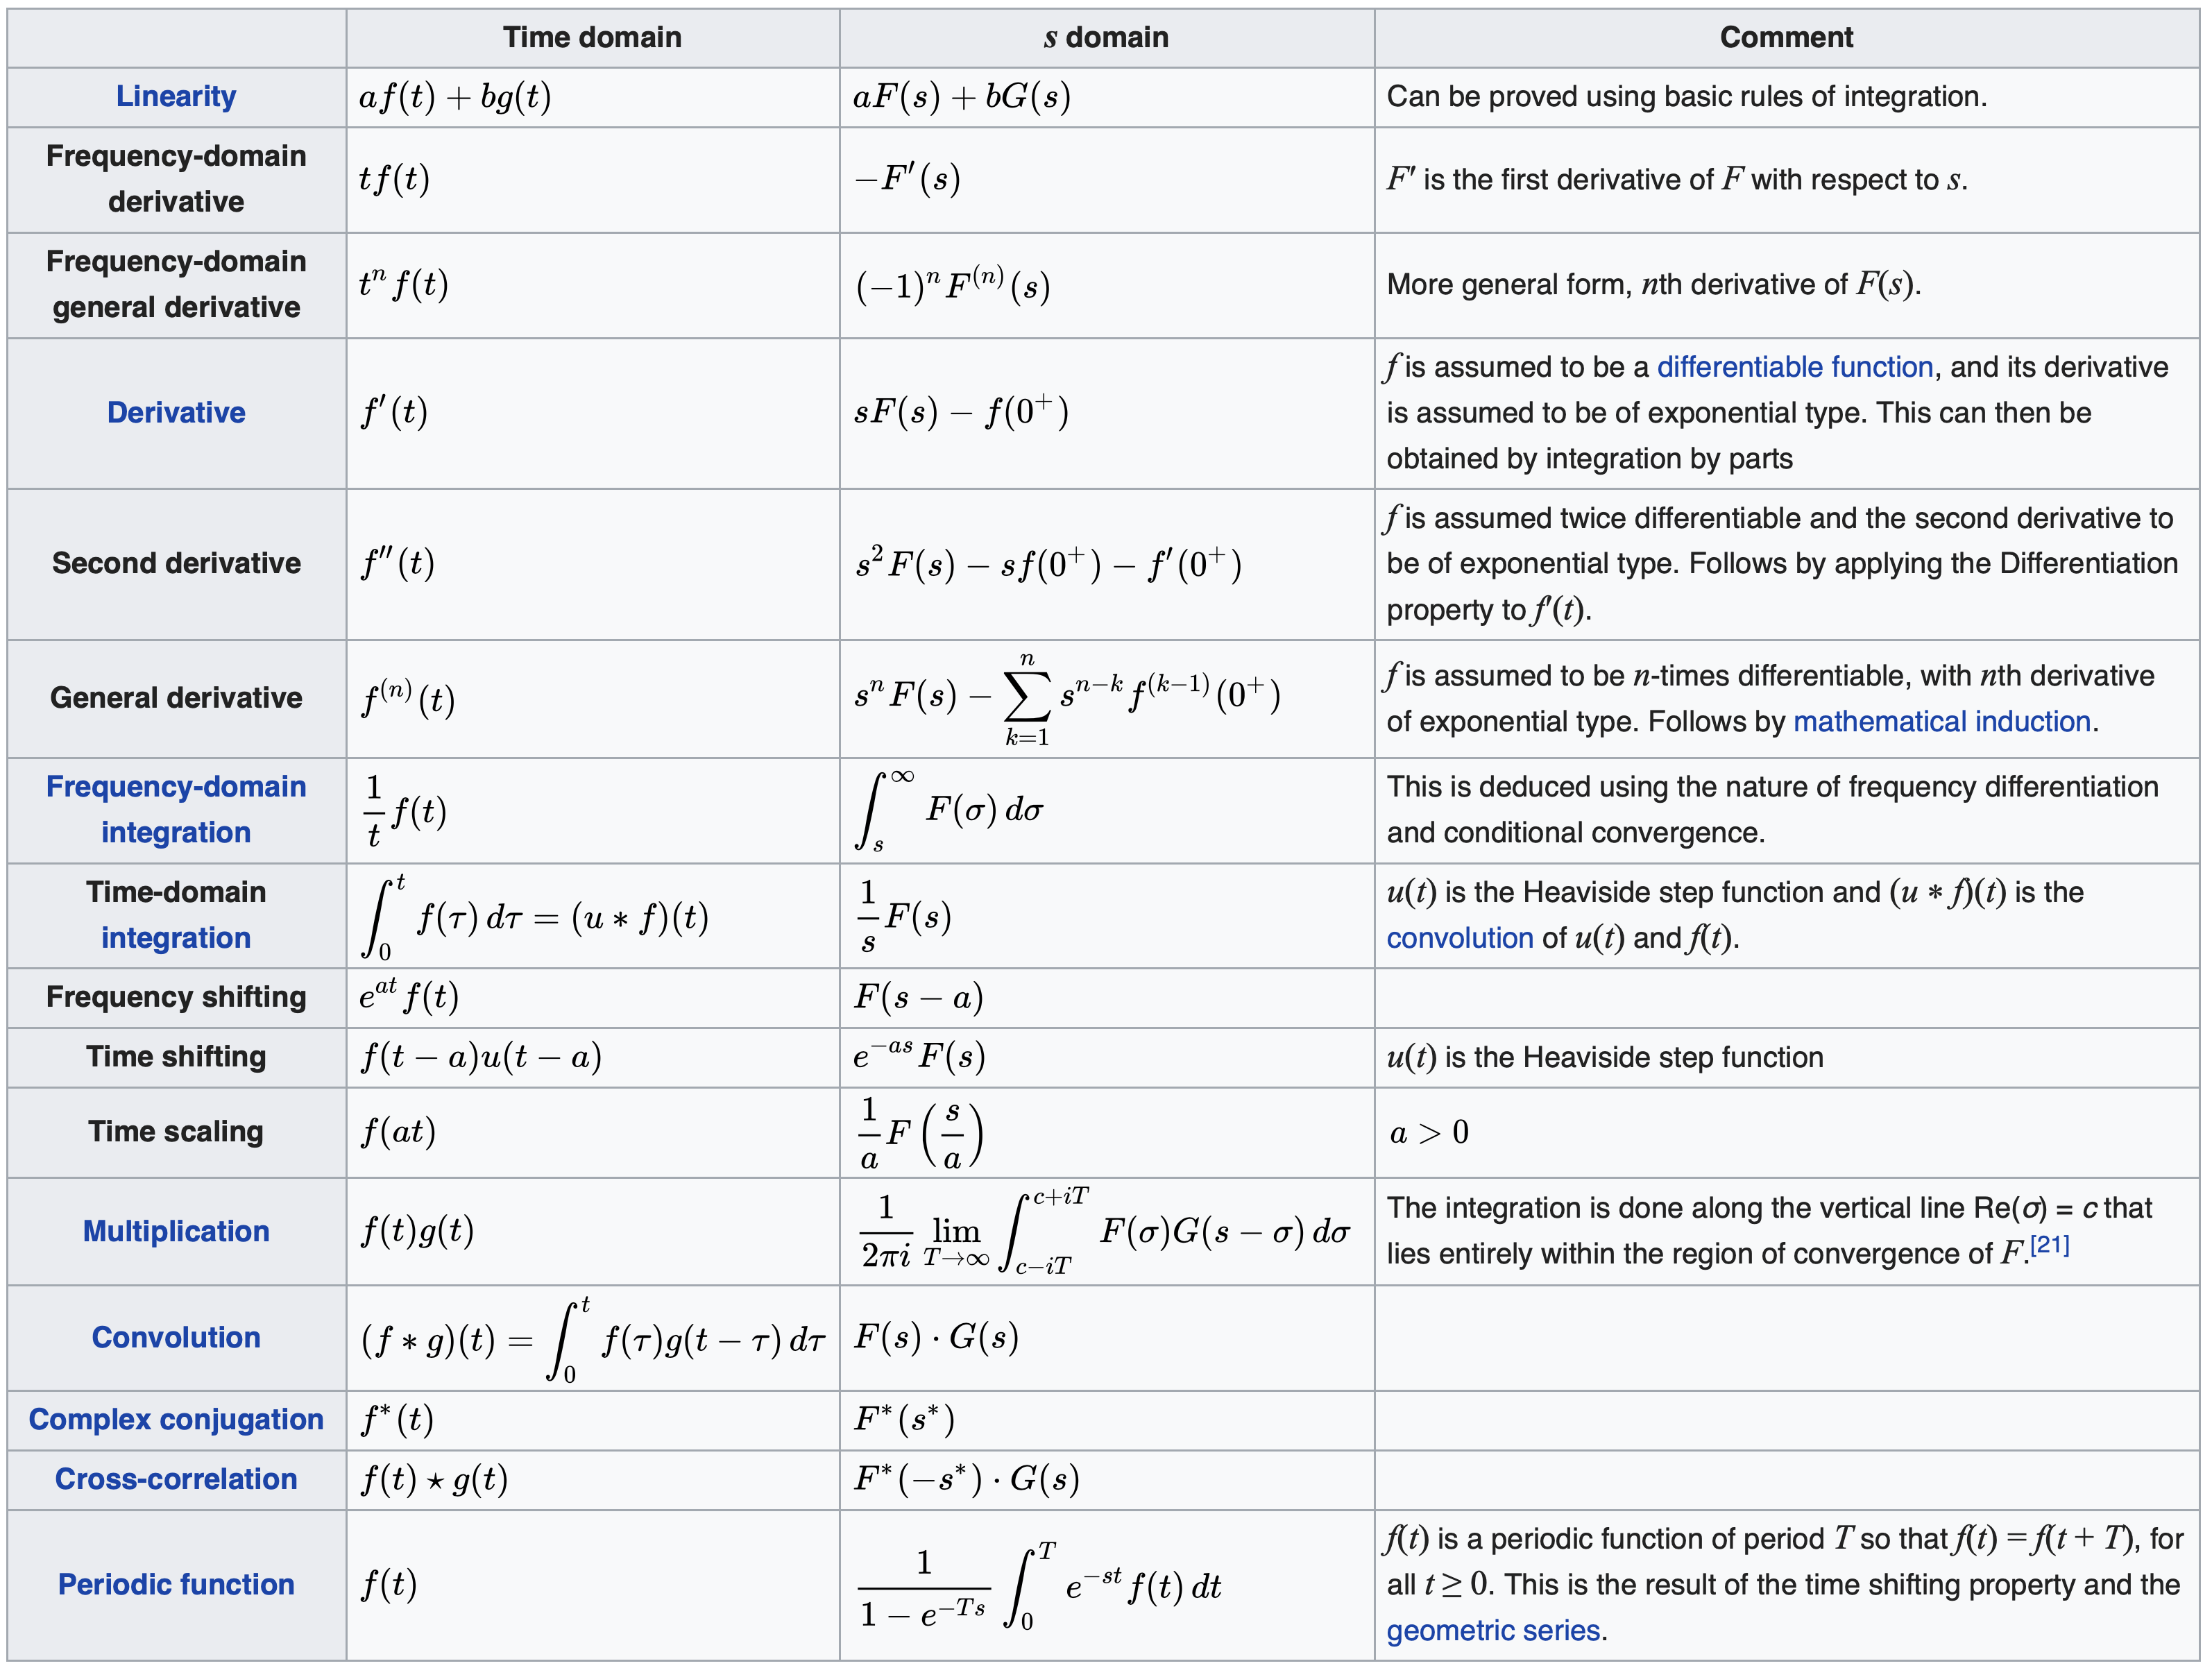
\includegraphics[width=.85\columnwidth]{laplace_table.png}
\caption{Table of Laplace Transform properties from the Wikipedia site.}
\label{fig:laplace_table}
\end{figure}
%%%%%%%%%%%%%%%%%%%%%%%%%%%%%%%%%%%%%%%%%%%%
%                 FIGURE                   %
%%%%%%%%%%%%%%%%%%%%%%%%%%%%%%%%%%%%%%%%%%%%
\begin{figure}[H]
\centering
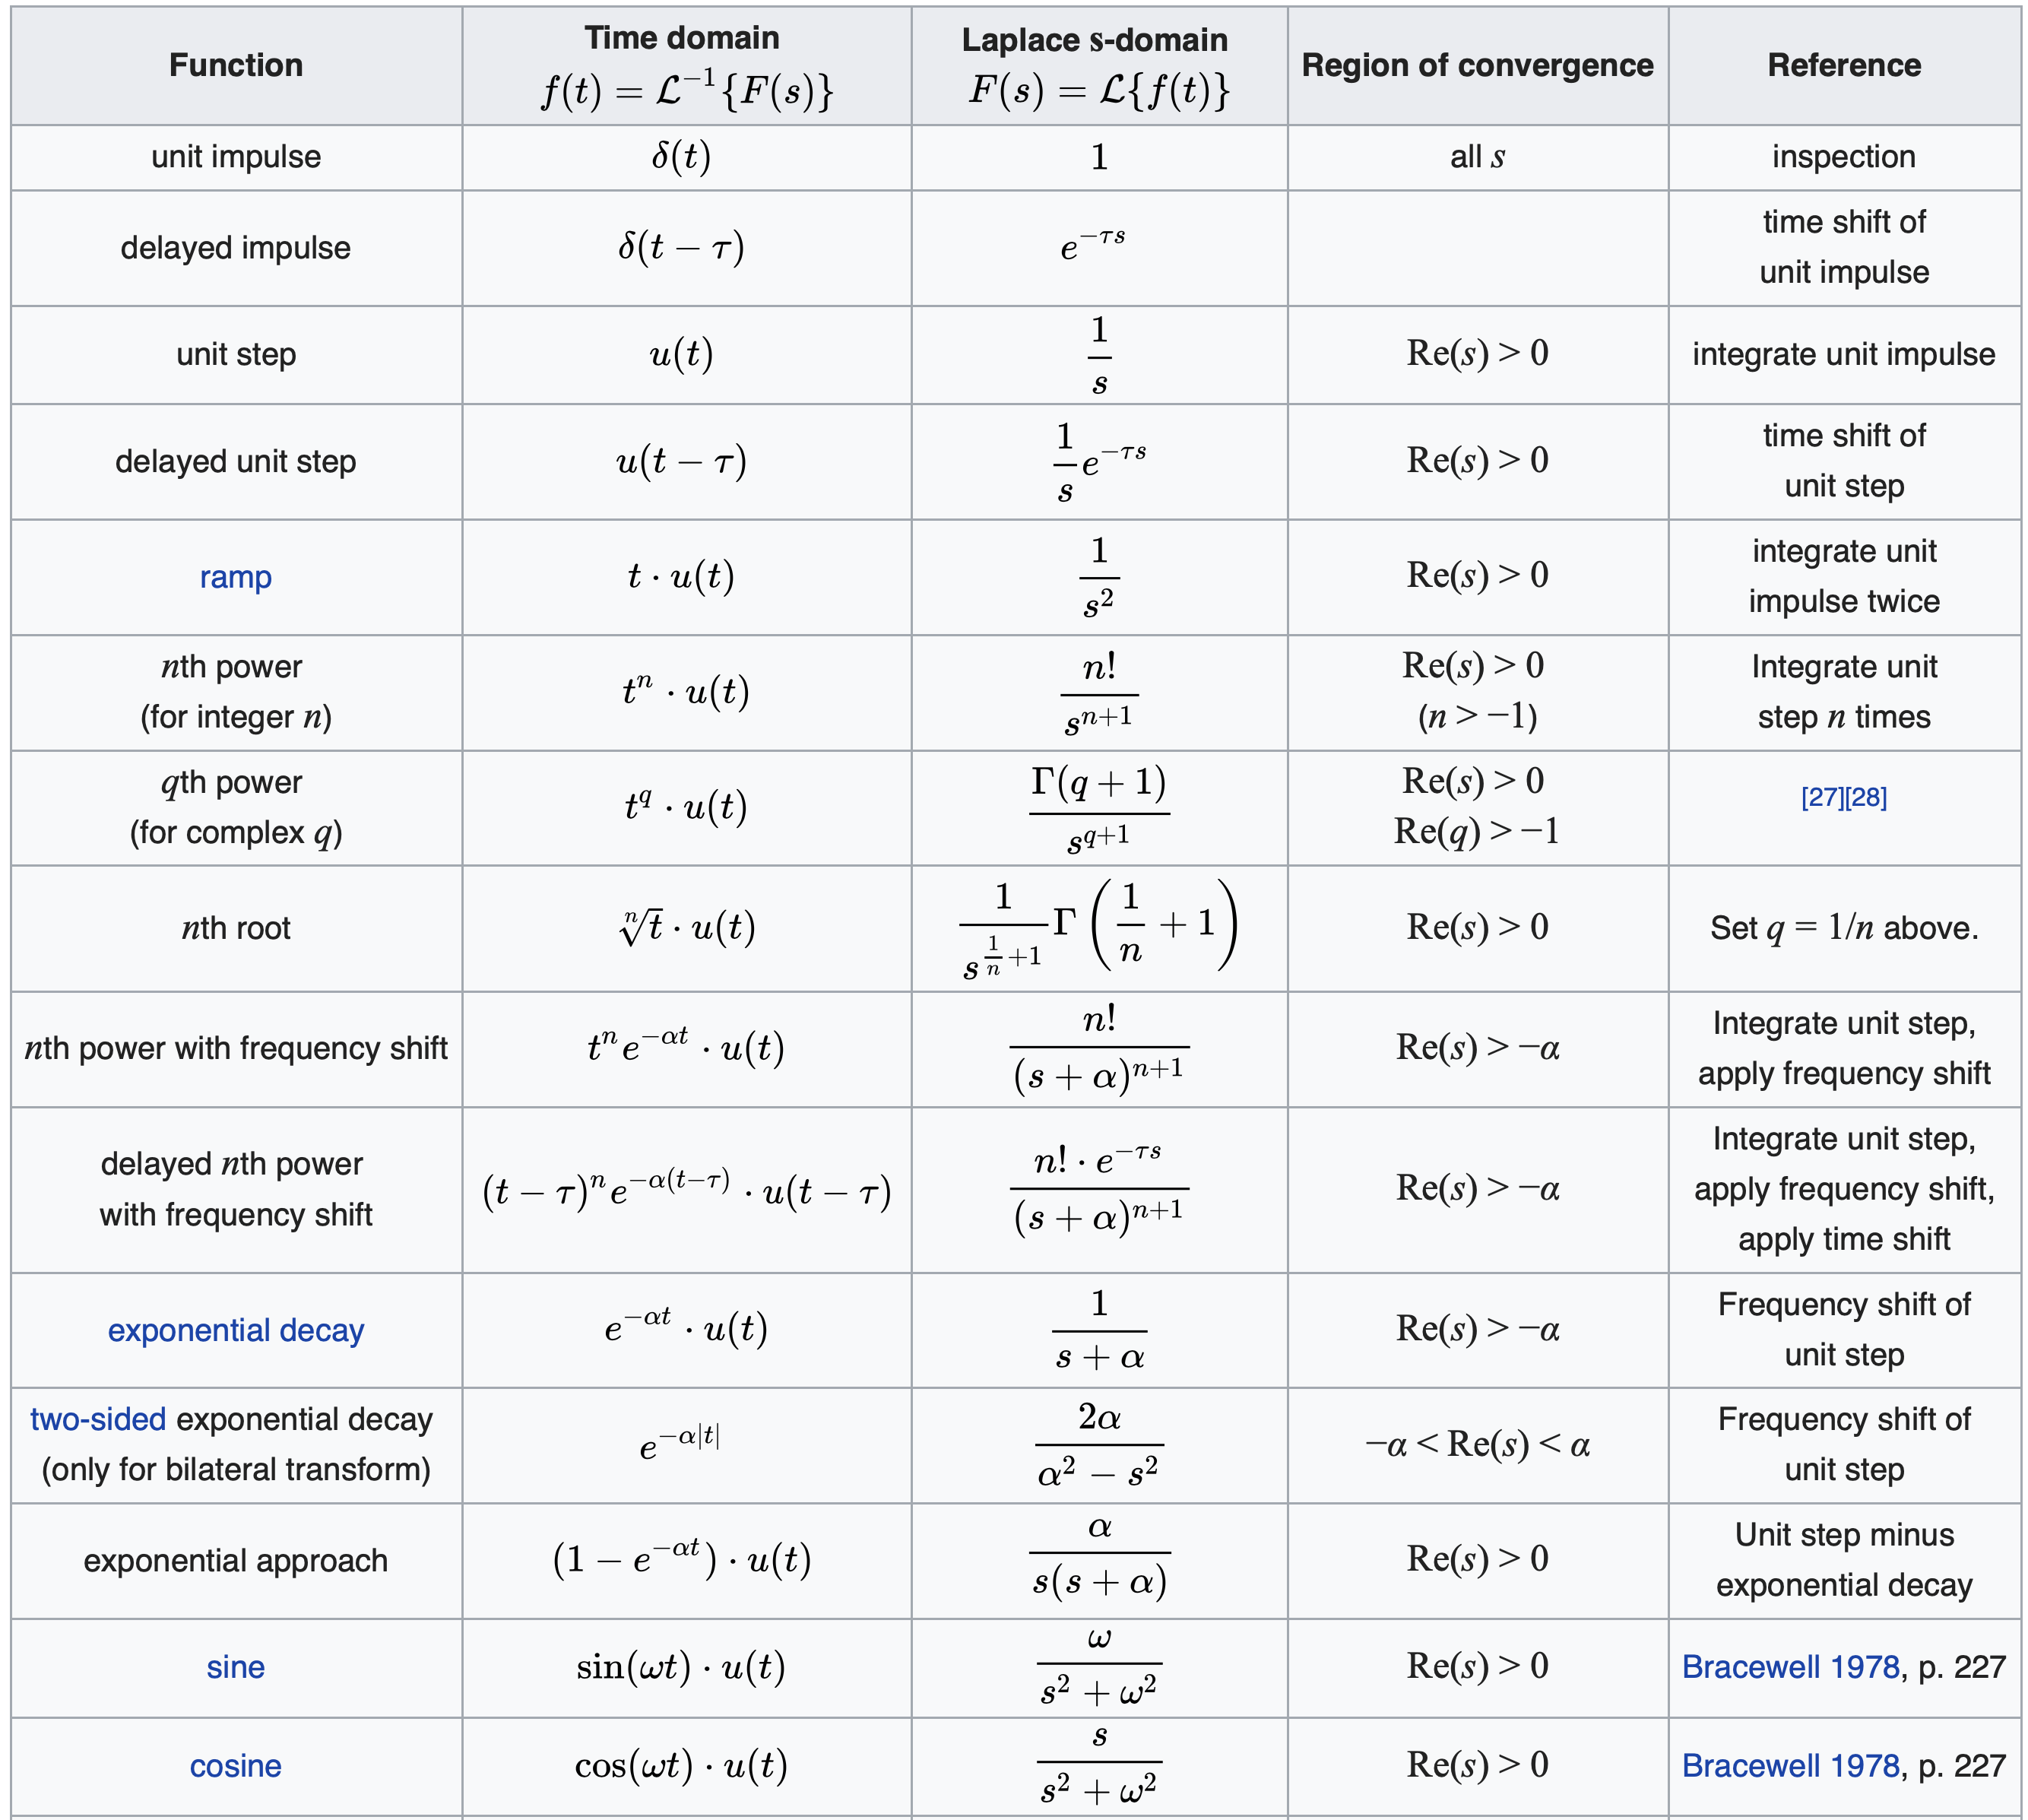
\includegraphics[width=.85\columnwidth]{laplace_transform.png}
\caption{Table of Laplace Transform pairs from the Wikipedia site.}
\label{fig:laplace_xform}
\end{figure}
%%%%%%%%%%%%%%%%%%%%%%%%%%%%%%%%%%%%%%%%%%%%
%             SUBSECTION 1.10.3            %
%%%%%%%%%%%%%%%%%%%%%%%%%%%%%%%%%%%%%%%%%%%%
\subsection{Fourier Series and Transform}
In previous courses, you may have learned that you can represent a periodic function in time as a \textbf{Fourier series}\index{Fourier series}
    \begin{equation}
        x(t) = \sum_{n = -\infty}^{\infty} c_n e^{j 2 \pi n f_0 t}
        \label{eq:fourier_series}
    \end{equation}
In this equation $f_0 = 1/T$ is the fundamental frequency of the function of period $T$.  For many practical signals of interest, we can go back and forth between the time or frequency domain, in the sense that the coefficients $c_n$ are a complete representation of the signal (invertable).  The FFT (\textbf{Fast Fourier Transform}\footnote{see Appendix~\ref{app:fft} for a review of the FFT}) is an efficient way to compute the Fourier Series.   We know that the magnitude of the coefficients $c_n$ determine the amount of power concentrated around a certain frequency.  If a function varies gradually in time with a time scale say less than $T$, then coefficients above $n =  f_0 T $ will be smaller in magnitude.

The Fourier Transform is a natural extension of the Fourier Series into the continuous time domain and it works for non-periodic functions (it has a line spectrum for periodic functions)
    \begin{equation}
        X(\omega)  = \mathcal{F} \left\{ x(t) \right\} =  \int_{-\infty}^{\infty} e^{-j \omega t} x(t) dt
    \end{equation}
And the inverse transform is given by
    \begin{equation}
        x(t) =  \mathcal{F}^{-1} \left\{ x(t) \right\} = \int_{-\infty}^{\infty} e^{j \omega t} X(f) df
    \end{equation}
For most signals, this is a well defined transformation allowing us to think of a signal in either the time domain or frequency domain. Notice that the Fourier Transform is related to the Laplace Transform by
    \begin{equation}
        \mathcal{F} \left\{ x(t) \right\}  = \left. X(s) \right|_{s = j\omega}  = X(j\omega)
    \end{equation}
This brings us full circle and shows that the frequency response $H(j\omega)$, the sinusoidal steady-state response, is in fact related to the Laplace Transform of the impulse response of our system.  While $H(s)$ is general, $H(j\omega)$, or the Fourier Transform of the impulse response, it a special case that applies to the periodic steady-state response.  
%%%%%%%%%%%%%%%%%%%%%%%%%%%%%%%%%%%%%%%%%%%%
%             SUBSECTION 1.10.4            %
%%%%%%%%%%%%%%%%%%%%%%%%%%%%%%%%%%%%%%%%%%%%
\subsection{Frequency Domain Interpretation}
If we transform the input function from the time domain to the frequency domain, then we can simply say that every frequency component in the input gets multiplied and phase shifted by the corresponding frequency domain component of the transfer function, as shown in \emph{Fig.~\ref{fig:freq_domain}}.
%%%%%%%%%%%%%%%%%%%%%%%%%%%%%%%%%%%%%%%%%%%%
%                 FIGURE                   %
%%%%%%%%%%%%%%%%%%%%%%%%%%%%%%%%%%%%%%%%%%%%
\begin{figure}[H]
\centering
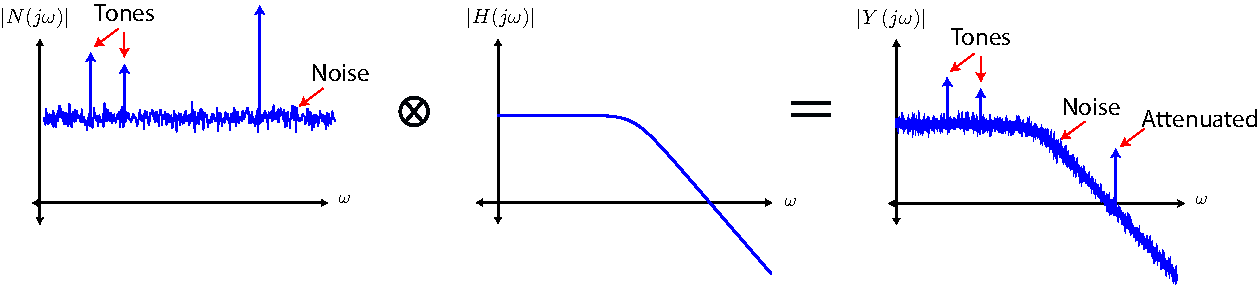
\includegraphics[width=\columnwidth]{sig_noise_freq.pdf}
\caption{The frequency domain representation of a signal plus noise (left).  The signal consists of tones (delta-functions in frequency domain) and noise (flat spectrum).  The signal is low-pass filtered, which is equivalent to multiplication by the frequency domain transfer function shown in the middle, resulting in the filtered signal and reduction in noise (right).}
\label{fig:freq_domain}
\end{figure}
%%%%%%%%%%%%%%%%%%%%%%%%%%%%%%%%%%%%%%%%%%%%
This follows from the properties of convolution in time becoming multiplication in the frequency domain.  Understanding a filter is much, much easier when is it analyzed in the frequency domain.  In this example we see a frequency domain representation of a signal with three tones, shown as Delta functions.  They are delta functions because the input signal consists of pure tones with a very long duration, and so all the energy is concentrated in these two frequency bands.  We also show that the signal is accompanied by "white noise", shown as a flat spectrum signal.  Although we have not proven this yet, it can be shown that noise is a wideband signal and can be modeled as a flat signal in the frequency domain.

If we low-pass filter the signal and noise, we expect that we will reduce the contribution of the noise.  In this example we suppose that the third tone is undesired, so we select the corner frequency of the filter just beyond the second tone, so that we do not attenuate the desired tones.  After filtering,   we would expect that the overall noise of the signal can be reduced without affecting the signals of interest.  This is shown by simply multiplying the frequency domain representation of the signal and noise with the filter response.  We see the noise contribution beyond the corner is reduced dramatically, and the third tone is also attenuated.
%%%%%%%%%%%%%%%%%%%%%%%%%%%%%%%%%%%%%%%%%%%%
%              SUB-SUBSECTION              %
%%%%%%%%%%%%%%%%%%%%%%%%%%%%%%%%%%%%%%%%%%%%
\subsubsection{Audio Example}
In this example, the input signal consists of a pure tone (261.626 Hz) and its third harmonic, which is delayed with respect to the fundamental.  Also, the signal is corrupted by a lot of noise content.  The signals of interest are shown in \emph{Fig.~\ref{fig:tones_time}}.  Now consider the signal + noise with noise power 10$\times$ lower (Signal-Noise Ratio (SNR) = 10 dB), as shown in \emph{Fig.~\ref{fig:sigplusnoise}}.
%%%%%%%%%%%%%%%%%%%%%%%%%%%%%%%%%%%%%%%%%%%%
%                 FIGURE                   %
%%%%%%%%%%%%%%%%%%%%%%%%%%%%%%%%%%%%%%%%%%%%
\begin{figure}[H]
\centering
\begin{tabular}{cc}
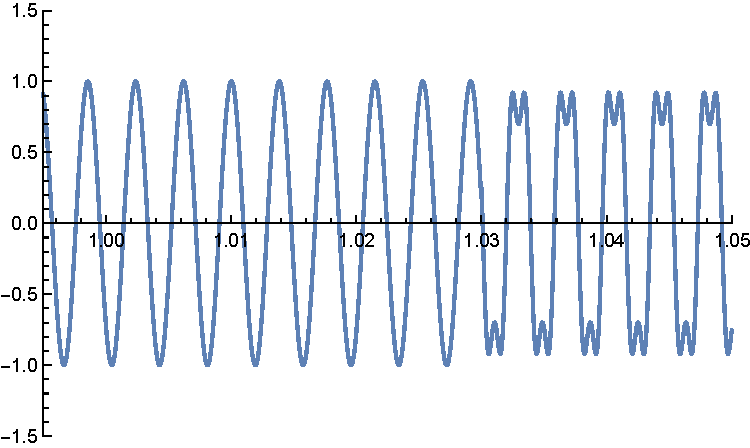
\includegraphics[width=.45\columnwidth]{tonesintime.pdf} &
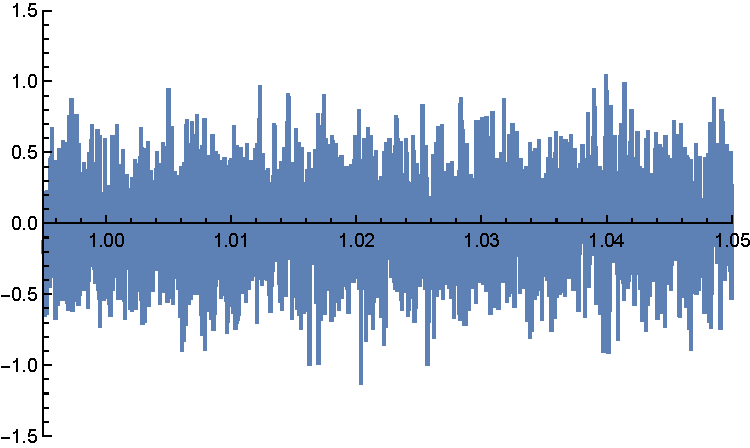
\includegraphics[width=.45\columnwidth]{noiseonly.pdf} \\
\end{tabular}
\caption{A audio signal consisting of a tone and the third harmonic (delayed by 1 second).  The signal will be added to the noisy signal shown on the right.}
\label{fig:tones_time}
\end{figure}
%%%%%%%%%%%%%%%%%%%%%%%%%%%%%%%%%%%%%%%%%%%%
%                 FIGURE                   %
%%%%%%%%%%%%%%%%%%%%%%%%%%%%%%%%%%%%%%%%%%%%
\begin{figure}[H]
\begin{center}
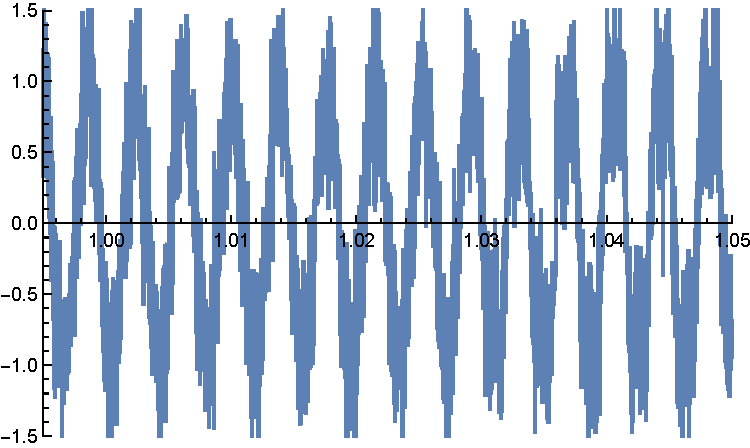
\includegraphics[width=.45\columnwidth]{signoise.pdf}
\end{center}
\caption{The noisy signal is shown.  The noise impacts both the amplitude and zero crossings of the signal.} \label{fig:sigplusnoise}
\end{figure}
%%%%%%%%%%%%%%%%%%%%%%%%%%%%%%%%%%%%%%%%%%%%
\newpage
\noindent
Click the following links to listen to the signals:
\vspace{0.15cm}
    \begin{itemize}
        \item{\href{http://rfic.eecs.berkeley.edu/~niknejad/photos/ee105/tones.mp3}{Tone + Third Harmonic, no noise}}
        \item{\href{http://rfic.eecs.berkeley.edu/~niknejad/photos/ee105/tones\_noise.mp3}{Signal + Noise}}
        \item{\href{http://rfic.eecs.berkeley.edu/~niknejad/photos/ee105/noise.mp3}{Just the "white" noise}}
    \end{itemize}	
\vspace{0.15cm}
Now if we filter the signal + noise, we can reduce the noise without impacting the signal (since the signal is mostly at low frequency in this case):
\vspace{0.15cm}
    \begin{itemize}
        \item{\href{http://rfic.eecs.berkeley.edu/~niknejad/photos/ee105/tones\_lpf.mp3}{Low-pass filtered signal + noise}}
    \end{itemize}
\vspace{0.15cm}
 This is used extensively in practice to improve the signal quality.  To improve the signal quality further, we build a \textbf{band-pass filter}\index{Filters!Band-pass} to pick out just the tone of interest.  The first filter picks up the first tone, and eliminates most of the noise.
\vspace{0.15cm}
    \begin{itemize}
        \item{\href{http://rfic.eecs.berkeley.edu/~niknejad/photos/ee105/tones\_bpf\_wC.mp3}{Band-pass filtered centered around first tone}}
    \end{itemize}
\vspace{0.15cm}
Now we apply a bandpass filter with a  wider passband, allowing both tones to pass.  We pickup both tones, but of course the downside is we hear more noise.
\vspace{0.15cm}
    \begin{itemize}
        \item{\href{http://rfic.eecs.berkeley.edu/~niknejad/photos/ee105/tones\_bpf.mp3}{Wideband filtered signal + noise}}
    \end{itemize}
%%%%%%%%%%%%%%%%%%%%%%%%%%%%%%%%%%%%%%%%%%%%
%             SUBSECTION 1.10.5            %
%%%%%%%%%%%%%%%%%%%%%%%%%%%%%%%%%%%%%%%%%%%%
\subsection{But Most Systems are Non-Linear ...?}
As we have demonstrated throughout this chapter, linear system theory is powerful and very useful for design and analysis.  But you may object and say that most real systems are non-linear, so why is this stuff useful?

When systems are non-linear, we often "linearize" them about an operating point, and use linear theory to understand the response to "small" perturbations.  We will be doing this extensively in this course.  Soon you will find that the silicon transistor and diodes are non-linear, so we will build "small-signal" models that are linear.  This is useful as long as the signals of interest don't deviate too much from the operating point.  If they do, we need non-linear techniques.  Even in these situations,  we can gain useful insights from the small-signal approximation, and it is the starting point for design and analysis.
%%%%%%%%%%%%%%%%%%%%%%%%%%%%%%%%%%%%%%%%%%%%%%%%%%%%%%%%%%%%%%%%%%%%%%%%%%%%%%%%%%%%%%%%
%%%%%%%%%%%%%%%%%%%%%%%%%%%%%%%%%%%%%%%%%%%%%%%%%%%%%%%%%%%%%%%%%%%%%%%%%%%%%%%%%%%%%%%%
%                                   SECTION 1.11                                       %
%%%%%%%%%%%%%%%%%%%%%%%%%%%%%%%%%%%%%%%%%%%%%%%%%%%%%%%%%%%%%%%%%%%%%%%%%%%%%%%%%%%%%%%%
%%%%%%%%%%%%%%%%%%%%%%%%%%%%%%%%%%%%%%%%%%%%%%%%%%%%%%%%%%%%%%%%%%%%%%%%%%%%%%%%%%%%%%%%
\section{Chapter Summary}
This chapter has taken us from the frequency domain AC style analysis to the time domain impulse response, and then all the way back full circle to the frequency domain transfer function.

Frequency response allows us to completely characterize a system using the sinusoidal response.  More generally, the frequency response is characterized by the complex exponential response $H(s)$.   The impulse response $h(t)$ completely characterizes a system in the time-domain, and we found a connection between the two approaches.   The transfer function $H(s)$ is the Laplace Transform of the impulse response $h(t)$.  The Fourier Transform is the Laplace transform evaluated on the imaginary axis, and AC circuit theory is how we calculate (or measure) the transfer function in practice.   Convolution in time simplifies to multiplication in the frequency domain (and vice versa).  Many concepts as calculations are easier to carry out in the frequency domain (filters), and as an engineer your intuition for the frequency domain will increase throughout your career.
 